% =========================================================================
% Recap del paper rifiutato (IEEE TCSS)
% "From Articles to Publishers". Solo recap di cosa e' stato fatto;
% le review si vedono nei messaggi successivi.
% Stile Madrid, poche voci per slide, una alla volta, con qualche figura.
% La parte statistica (chi-quadro) e' spiegata passo passo in modo semplice.
% Build: tectonic recap_paper.tex
% =========================================================================
\documentclass[aspectratio=169]{beamer}
\usetheme{Madrid}
\usecolortheme{whale}
\usepackage[T1]{fontenc}
\usepackage{graphicx}
\usepackage{booktabs}
\usepackage{xcolor}
\usepackage{tikz}
\graphicspath{{../../Paper/OldPaperRejected/img/}{./}}

\beamertemplatenavigationsymbolsempty
\setbeamercovered{invisible}
\setbeamertemplate{caption}{\insertcaption}
\newcommand{\hl}[1]{\textbf{#1}}
\newenvironment{johnblock}{\begin{exampleblock}{\footnotesize Commento di John}\footnotesize}{\end{exampleblock}}
\newenvironment{claudeblock}{\setbeamercolor{block title}{fg=white,bg=gray!65!black}\setbeamercolor{block body}{bg=gray!12}\begin{block}{\footnotesize Commento di Claude}\footnotesize}{\end{block}}
\newcommand{\divider}[2]{%
  \begin{frame}[plain]
    \vfill
    \begin{center}
      {\color{dividerblue}\Huge\textbf{#1}}\\[0.8em]
      {\large #2}
    \end{center}
    \vfill
  \end{frame}}
\definecolor{wrongred}{RGB}{176,0,32}
\definecolor{dividerblue}{RGB}{28,42,92}
\newcommand{\wrong}[1]{\textcolor{wrongred}{#1}}

\title[Verso Web Science 2027]{Verso Web Science 2027}
\subtitle{Riprendere il paper bocciato: recap del lavoro e prossimi passi}
\author[Riunione di gruppo]{Riunione di gruppo}
\institute[]{IMT Lucca \& IIT-CNR Pisa}
\date{}

\begin{document}

% ---------------------------------------------------------------- titolo
\begin{frame}
  \titlepage
\end{frame}

% ---------------------------------------------------------------- divider: recap
\divider{Recap del paper bocciato}{non la versione sottomessa a IR for Good}

% ---------------------------------------------------------------- dati
\begin{frame}{Dati}
  \begin{columns}[c]
    \begin{column}{0.52\textwidth}
      \begin{itemize}[<+->]
        \setlength\itemsep{0.8em}
        \item Scraping con \hl{newspaper3k}
        \item 439 editori, 19.476 articoli politici in inglese
        \item Etichette \hl{NewsGuard}: 5 livelli $l_1$--$l_5$ (da 0--100)
        \item Ogni articolo \hl{eredita} l'etichetta del suo editore
      \end{itemize}
    \end{column}
    \begin{column}{0.48\textwidth}
      \visible<3->{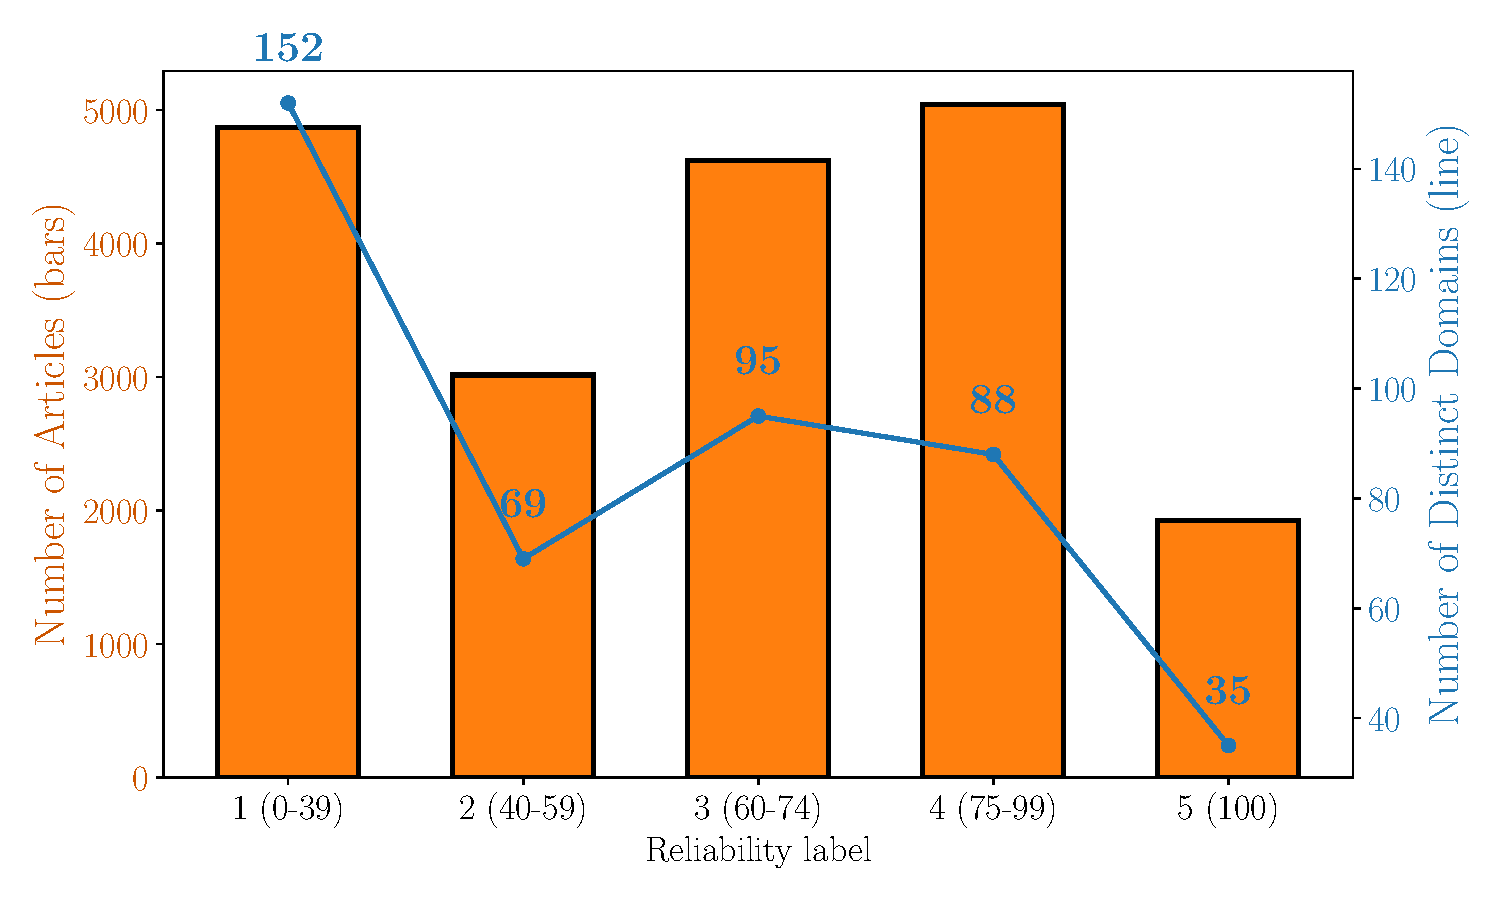
\includegraphics[width=\linewidth]{dataset_distribution.pdf}}
    \end{column}
  \end{columns}
\end{frame}

% ---------------------------------------------------------------- classificazione
\begin{frame}{Classificazione --- livello articolo}
  \begin{columns}[c]
    \begin{column}{0.5\textwidth}
      \begin{itemize}[<+->]
        \setlength\itemsep{0.8em}
        \item Quattro transformer: \hl{BERT, RoBERTa, Llama, Mistral}
        \item Encoder full fine-tuning, decoder con \hl{LoRA}
        \item Input \hl{256 token} (1024 per Mistral)
        \item Split \hl{publisher-disjoint}: editori di test mai visti
      \end{itemize}
    \end{column}
    \begin{column}{0.5\textwidth}
      \visible<5->{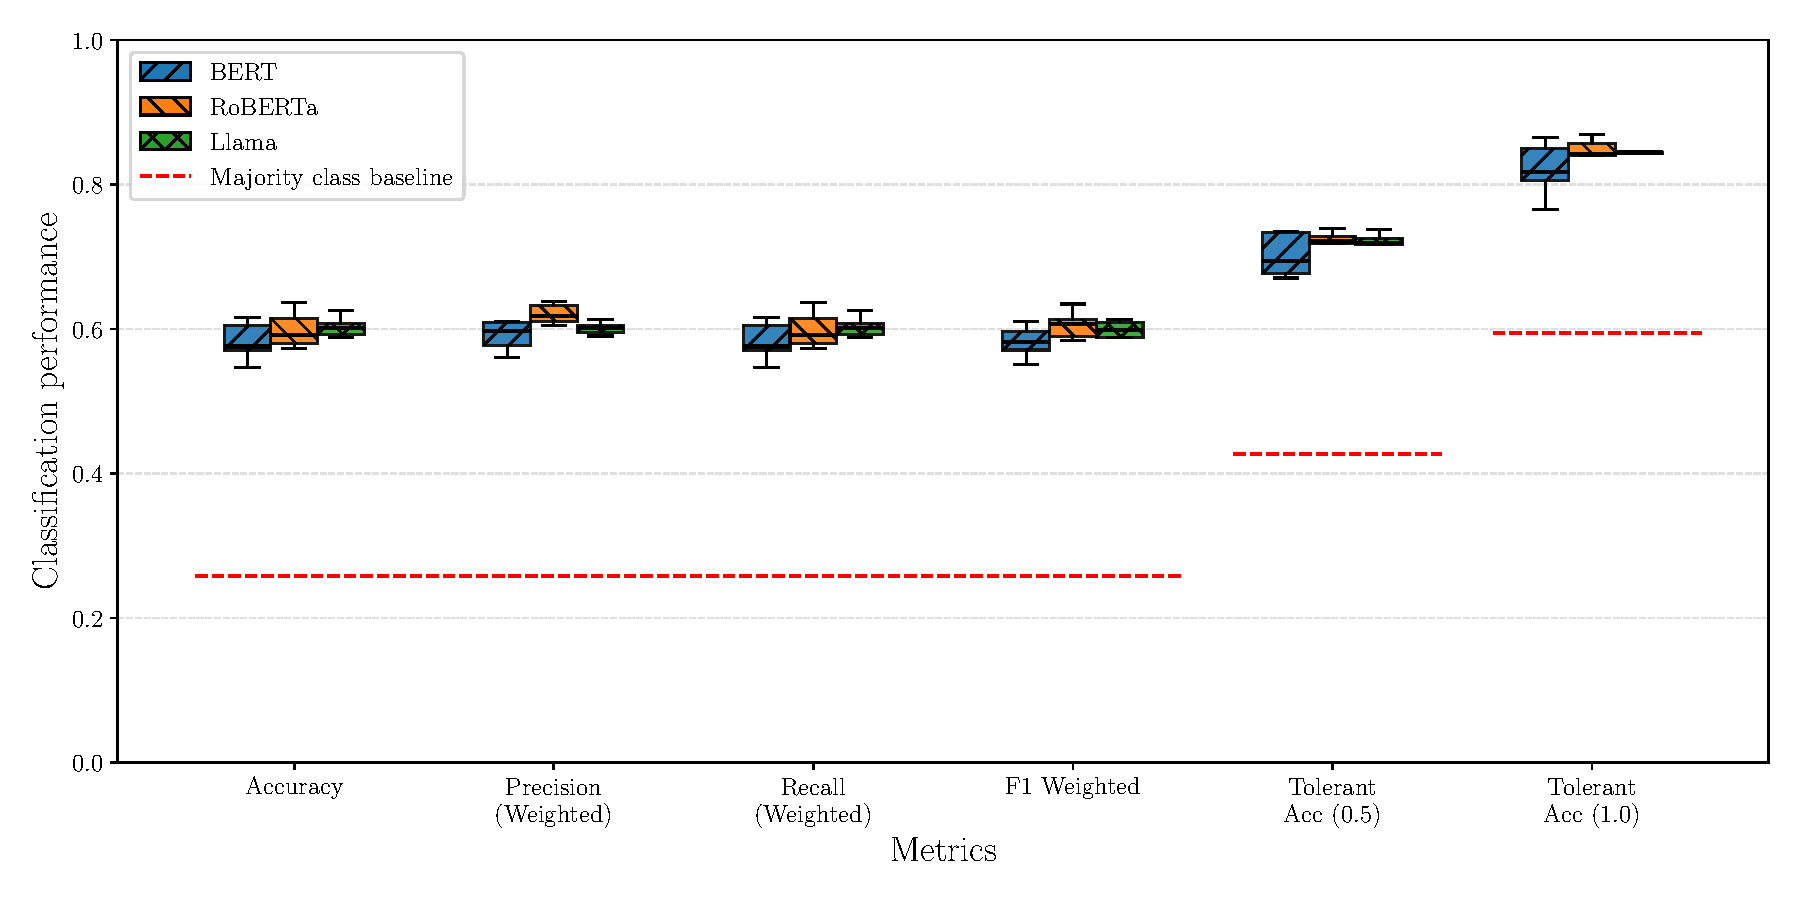
\includegraphics[width=\linewidth]{results_boxplot_baselines.pdf}}
    \end{column}
  \end{columns}
\end{frame}

% ---------------------------------------------------------------- aggregazione
\begin{frame}{Aggregazione --- livello editore}
  \begin{columns}[c]
    \begin{column}{0.5\textwidth}
      \begin{itemize}[<+->]
        \setlength\itemsep{0.9em}
        \item Dall'articolo all'editore con \hl{majority voting}
        \item Si usano \hl{tutti} gli articoli della testata: nessun cap in aggregazione (fino a 200, mediana $\sim$34)
        \item Valutazione su editori \hl{mai visti} in addestramento
      \end{itemize}
    \end{column}
    \begin{column}{0.5\textwidth}
      \visible<4->{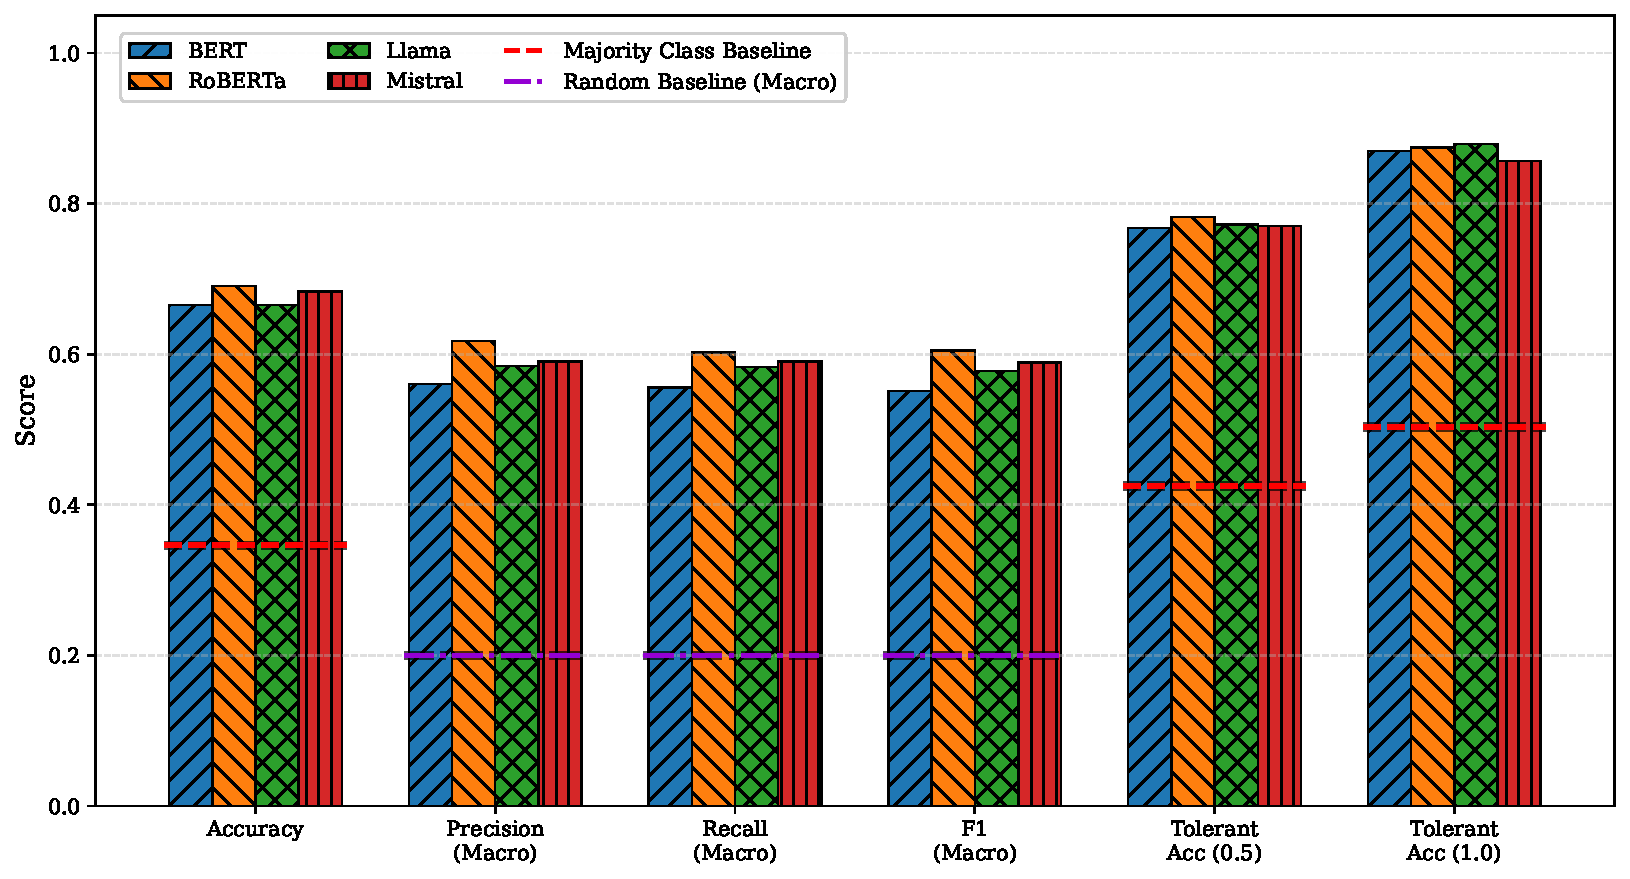
\includegraphics[width=\linewidth]{domain_metrics_comparison.pdf}}
    \end{column}
  \end{columns}
\end{frame}

% ================================================================
%  ANALISI DELL'ERRORE (livello di affidabilita')
% ================================================================

% ---------------------------------------------------------------- motivazione errore
\begin{frame}{Perch\'e analizziamo gli errori}
  \vfill
  \begin{itemize}[<+->]
    \setlength\itemsep{0.9em}
    \item Oltre alle metriche aggregate, vogliamo capire \hl{come} e \hl{perch\'e} i modelli sbagliano
    \item[] {\small\itshape ``Beyond aggregate performance, we investigate how and why models fail.''}
    \item Obiettivo: trovare \hl{debolezze strutturali} --- su quali livelli sbaglia e se sovra/sottostima
    \item[] {\small\itshape ``To detect structural weaknesses\dots''}
  \end{itemize}
  \vfill
\end{frame}

% ---------------------------------------------------------------- errore: per livello
\begin{frame}{Analisi dell'errore --- per livello}
  \begin{columns}[c]
    \begin{column}{0.5\textwidth}
      \begin{itemize}[<+->]
        \setlength\itemsep{0.9em}
        \item \hl{Error rate} per ogni livello di affidabilit\`a
        \item $l_1$: errore pi\`u \hl{basso} ($<20\%$)
        \item $l_5$: errore pi\`u \hl{alto} ($>70\%$), spesso confuso con $l_4$
        \item $l_2$ sopra il 50\%, $l_3$ intorno al 35\%
        \item[] {\small\itshape Sappiamo solo dove sbaglia di pi\`u o di meno, non perch\'e.}
      \end{itemize}
    \end{column}
    \begin{column}{0.5\textwidth}
      \visible<2->{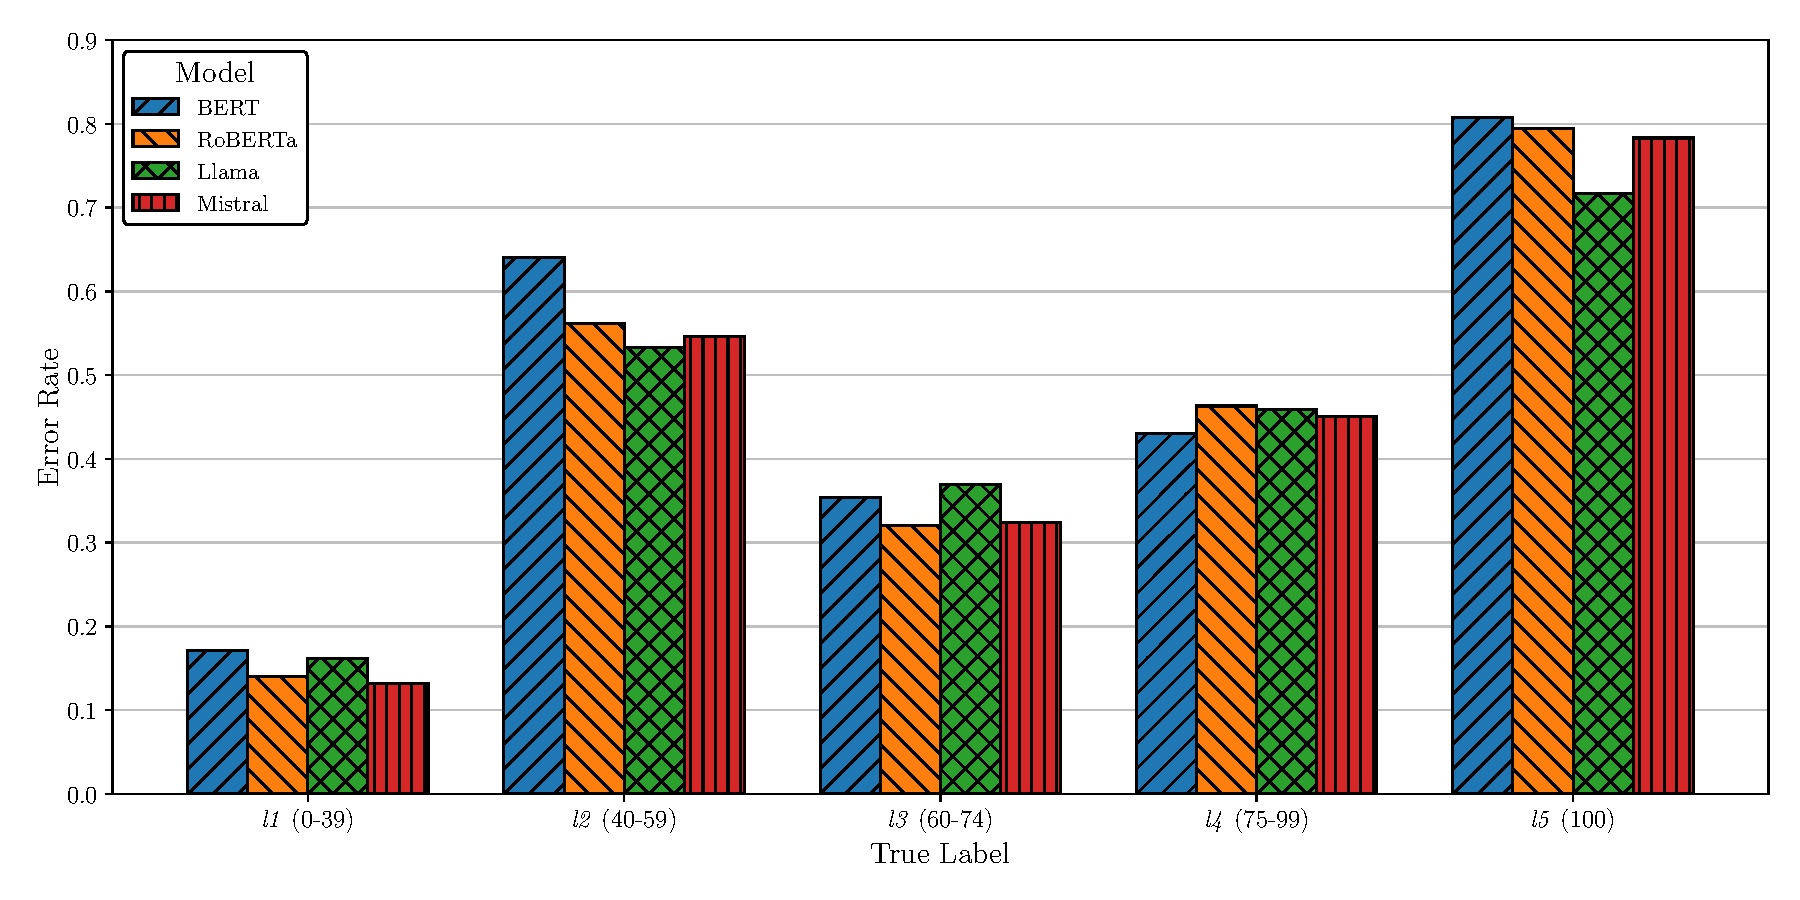
\includegraphics[width=\linewidth]{error_rate_analysis.pdf}}
    \end{column}
  \end{columns}
\end{frame}

% ---------------------------------------------------------------- errore: direzione per livello
\begin{frame}{Analisi dell'errore --- direzione}
  \begin{columns}[c]
    \begin{column}{0.5\textwidth}
      \begin{itemize}[<+->]
        \setlength\itemsep{0.9em}
        \item \hl{Mean Error Direction}: l'errore \emph{sovrastima} ($+$) o \emph{sottostima} ($-$) l'affidabilit\`a
        \item Livelli \hl{bassi sovrastimati}, livelli \hl{alti sottostimati}
        \item Gli errori ``tirano verso il \hl{centro}'' della scala
      \end{itemize}
    \end{column}
    \begin{column}{0.5\textwidth}
      \visible<2->{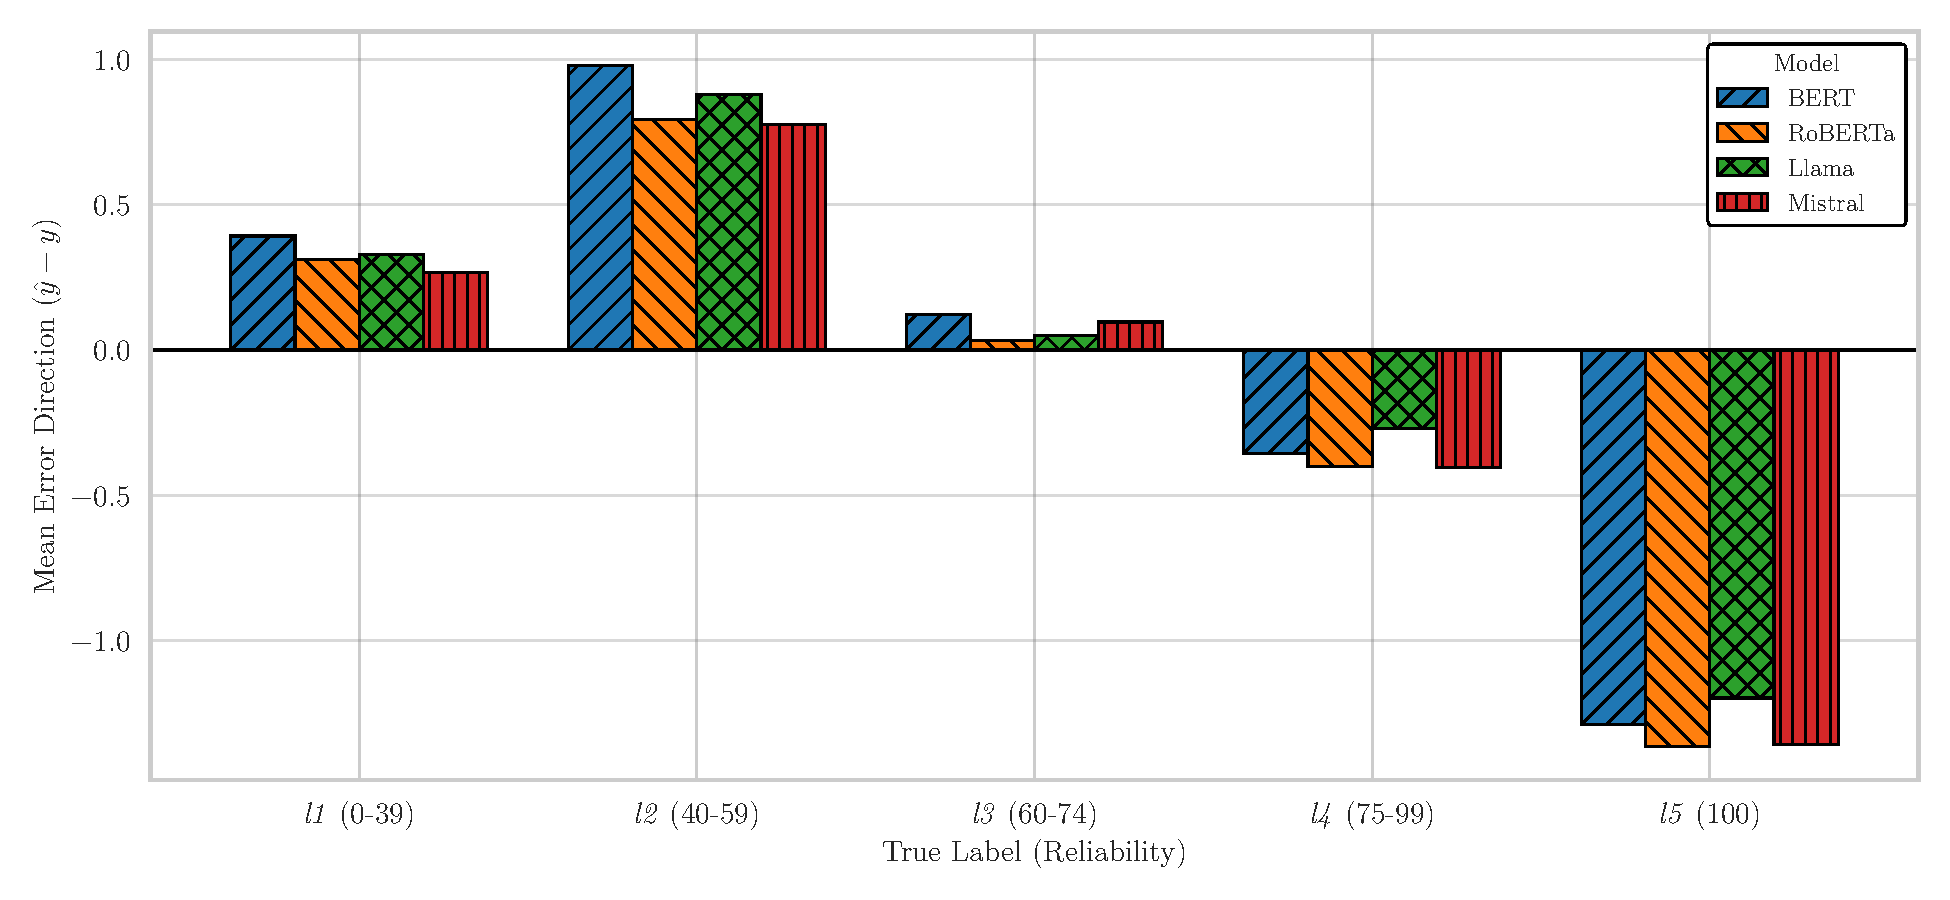
\includegraphics[width=\linewidth]{mean_error_direction.pdf}}
    \end{column}
  \end{columns}
\end{frame}

% ================================================================
%  ANALISI DEGLI ERRORI PER BIAS POLITICO
% ================================================================

% ---------------------------------------------------------------- motivazione bias
\begin{frame}{Perch\'e analizziamo il bias politico}
  \vfill
  \begin{itemize}[<+->]
    \setlength\itemsep{0.9em}
    \item Vogliamo sapere se il modello \hl{tratta allo stesso modo} tutto lo spettro politico, o se \hl{penalizza} certi orientamenti
    \item[] {\small\itshape ``\dots determine if the models exhibit political bias\dots whether the models treat all sides of the political spectrum equally or if they penalize specific orientations.''}
    \item Serve una valutazione \hl{bias-aware}: un sistema in uso con bias politico pu\`o fare danni
    \item[] {\small\itshape ``\dots the need for bias-aware evaluation protocols\dots''}
  \end{itemize}
  \vfill
\end{frame}

% ---------------------------------------------------------------- bias: distribuzione
\begin{frame}{Bias politico --- distribuzione dei dati}
  \begin{columns}[c]
    \begin{column}{0.5\textwidth}
      \begin{itemize}[<+->]
        \setlength\itemsep{0.9em}
        \item Orientamento ereditato dall'editore (analisi \emph{a posteriori})
        \item Dentro ogni orientamento, come si distribuiscono i livelli
        \item Distribuzione molto \hl{sbilanciata} (propriet\`a del sistema mediatico)
        \item Per questo gli error rate si calcolano \hl{classe per classe}
      \end{itemize}
    \end{column}
    \begin{column}{0.5\textwidth}
      \visible<2->{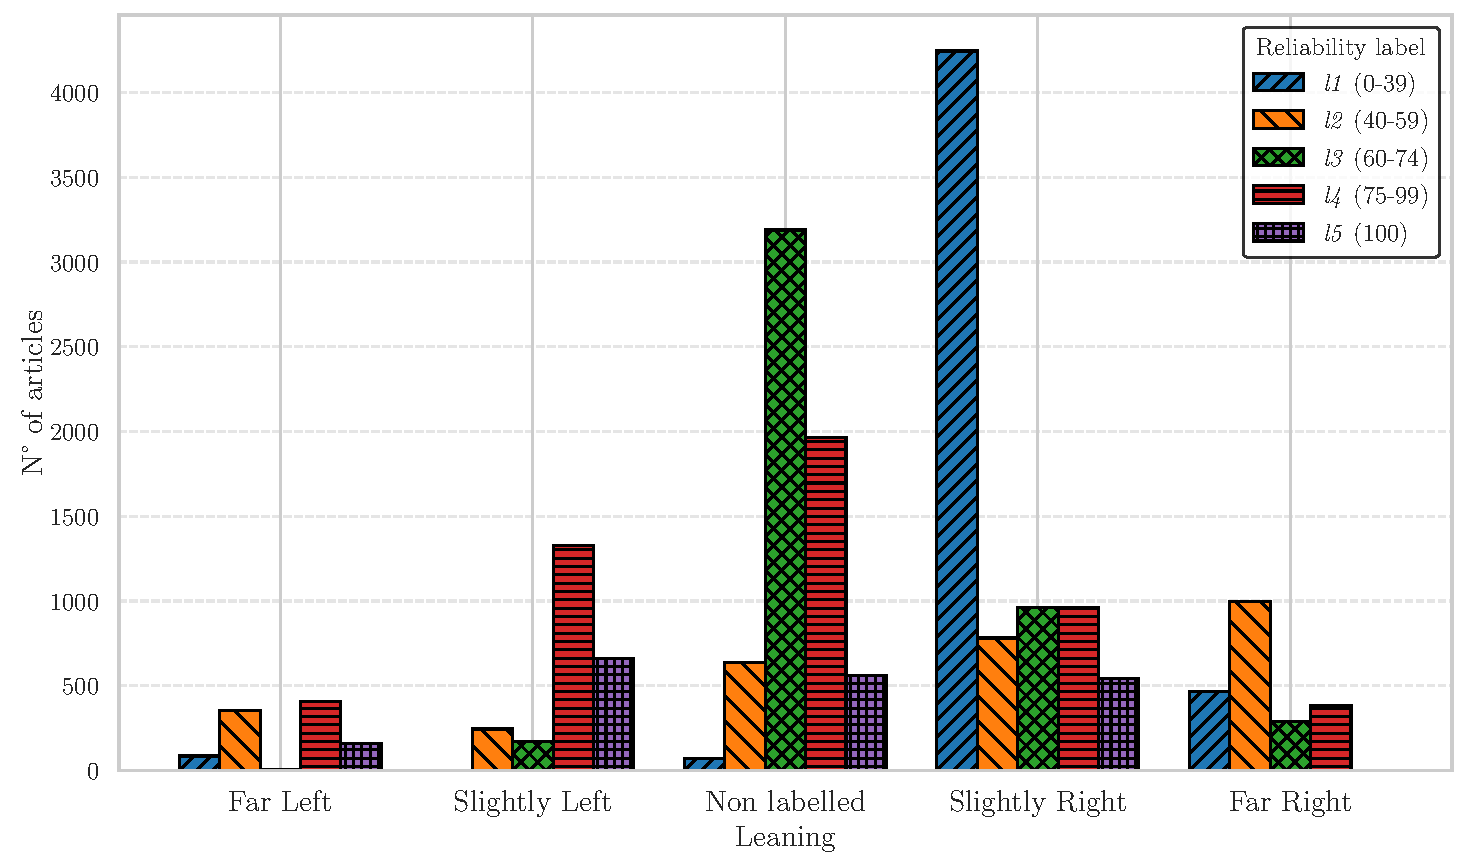
\includegraphics[width=\linewidth]{orientationDistributionInverted.pdf}}
    \end{column}
  \end{columns}
\end{frame}

% ---------------------------------------------------------------- bias: error rate
\begin{frame}{Bias politico --- error rate}
  \begin{columns}[c]
    \begin{column}{0.5\textwidth}
      \begin{itemize}[<+->]
        \setlength\itemsep{0.9em}
        \item \hl{Error rate} per orientamento politico
        \item Gli estremi (\hl{far left}, \hl{far right}) sbagliano molto di pi\`u
        \item Slightly right e non labelled sbagliano \hl{meno}
      \end{itemize}
    \end{column}
    \begin{column}{0.5\textwidth}
      \visible<2->{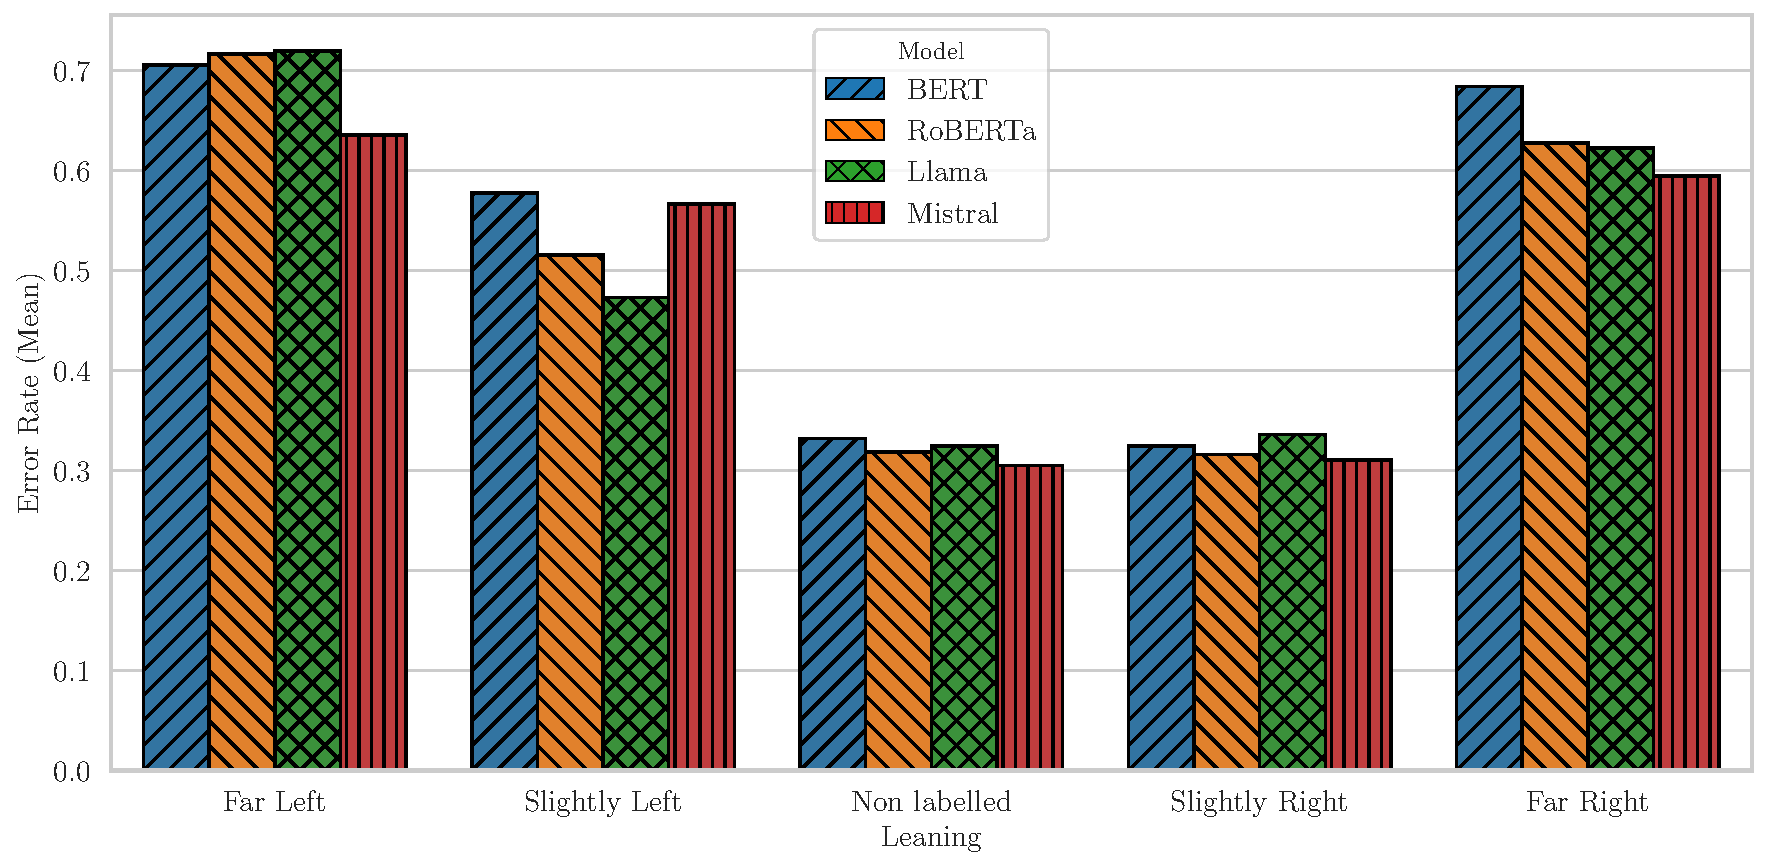
\includegraphics[width=\linewidth]{politicalErrorRates.pdf}}
    \end{column}
  \end{columns}
\end{frame}

% ---------------------------------------------------------------- bias: direzione
\begin{frame}{Bias politico --- direzione dell'errore}
  \begin{columns}[c]
    \begin{column}{0.5\textwidth}
      \begin{itemize}[<+->]
        \setlength\itemsep{0.9em}
        \item \hl{Mean Error Direction} per orientamento
        \item Estremi (far left, far right) \hl{sovrastimati}
        \item Slightly left \hl{sottostimato}
        \item Slightly right e non labelled: deviazioni piccole
      \end{itemize}
    \end{column}
    \begin{column}{0.5\textwidth}
      \visible<2->{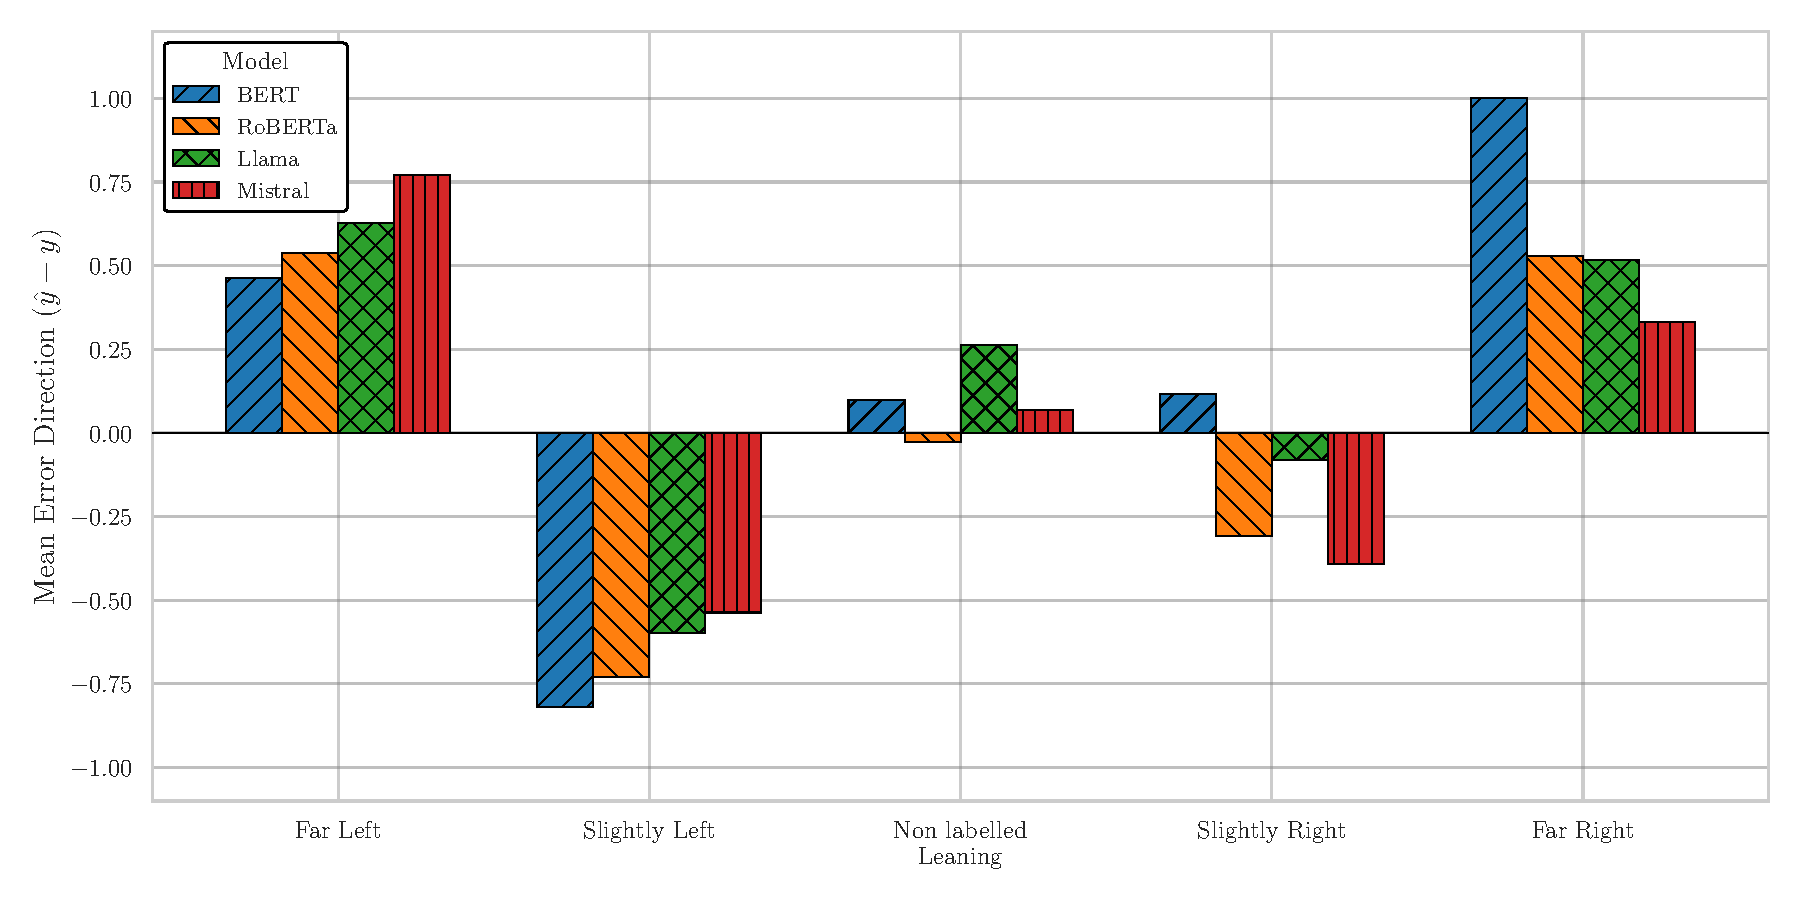
\includegraphics[width=\linewidth]{politicalErrorsDirection.pdf}}
    \end{column}
  \end{columns}
\end{frame}

% ---------------------------------------------------------------- stat: la domanda
\begin{frame}{\`E un vero legame o \`e un caso?}
  \vfill
  \begin{itemize}[<+->]
    \setlength\itemsep{1.0em}
    \item Vediamo error rate diversi tra gli orientamenti.
    \item Ma potrebbe essere solo \hl{rumore} dei dati.
    \item Serve un \hl{test statistico} che dica: questo legame \`e reale?
  \end{itemize}
  \vfill
  \onslide<4->{\begin{center}\small Strumento usato: il \hl{test del chi-quadro ($\chi^2$) di indipendenza}.\end{center}}
\end{frame}

% ---------------------------------------------------------------- stat: tabella contingenza
\begin{frame}{Passo 1 --- mettiamo gli errori in tabella}
  \begin{columns}[c]
    \begin{column}{0.46\textwidth}
      \begin{itemize}[<+->]
        \setlength\itemsep{0.8em}
        \item Per ogni orientamento contiamo \hl{giusti} e \hl{sbagliati}
        \item \`E la \hl{tabella di contingenza}
        \item Agli estremi gli \wrong{sbagliati} superano i giusti
      \end{itemize}
    \end{column}
    \begin{column}{0.54\textwidth}
      \onslide<2->{%
      \footnotesize
      \begin{center}
      \begin{tabular}{lrr}
        \toprule
        \textbf{Orientamento} & \textbf{Giusti} & \textbf{\wrong{Sbagliati}} \\
        \midrule
        Far Left       & 299  & \wrong{716}  \\
        Slightly Left  & 1018 & \wrong{1389} \\
        Non labelled   & 4292 & 2130 \\
        Slightly Right & 5062 & 2428 \\
        Far Right      & 678  & \wrong{1464} \\
        \bottomrule
      \end{tabular}
      \end{center}
      \scriptsize\centering (esempio: BERT)
      }
    \end{column}
  \end{columns}
\end{frame}

% ---------------------------------------------------------------- stat: idea del chi2
\begin{frame}{Passo 2 --- l'idea del chi-quadro}
  \vfill
  \begin{itemize}[<+->]
    \setlength\itemsep{0.9em}
    \item Immaginiamo che l'orientamento \hl{non c'entri} con gli errori.
    \item Allora ogni gruppo dovrebbe sbagliare \hl{nella stessa proporzione} (circa la media, $\sim$42\%).
    \item Il $\chi^2$ misura \hl{quanto} gli errori \emph{osservati} si allontanano da questo scenario ``senza legame''.
    \item Pi\`u grande \`e lo scarto $\rightarrow$ $\chi^2$ grande $\rightarrow$ pi\`u probabile che un legame ci sia.
  \end{itemize}
  \vfill
\end{frame}

\begin{frame}{Passo 2 --- quanto vale il nostro $\chi^2$}
  \vfill
  \begin{itemize}[<+->]
    \setlength\itemsep{0.8em}
    \item Se \hl{non} ci fosse nessun legame, il $\chi^2$ starebbe intorno a \hl{4} (un valore che dipende solo dalla grandezza della tabella)
    \item Per puro caso supererebbe \hl{9,5} solo 1 volta su 20: \`e la soglia classica
    \item Il nostro: \hl{1.208--1.684}, a seconda del modello
    \item[] {\small\itshape Oltre cento volte la soglia: lontanissimo dallo scenario ``senza legame''.}
    \item Attenzione: il $\chi^2$ cresce con il \hl{numero di dati} (qui 19.476 articoli): per giudicare la \emph{forza} del legame serve Cram\'er's V (Passo 4)
  \end{itemize}
  \vfill
\end{frame}

% ---------------------------------------------------------------- stat: p-value
\begin{frame}{Passo 3 --- il $p$-value}
  \vfill
  \begin{itemize}[<+->]
    \setlength\itemsep{0.9em}
    \item Un $\chi^2$ grande potrebbe capitare \hl{per caso}?
    \item Il \hl{$p$-value} \`e la probabilit\`a di vedere uno scarto cos\`i grande \emph{se non ci fosse nessun legame}.
    \item $p$ piccolissimo (es. $p<0.001$) $\rightarrow$ quasi impossibile che sia un caso.
    \item Quindi il legame \`e \hl{reale}, non fortuna.
  \end{itemize}
  \vfill
\end{frame}

% ---------------------------------------------------------------- stat: Cramer V
\begin{frame}{Passo 4 --- quanto \`e forte? (Cram\'er's V)}
  \vfill
  \begin{itemize}[<+->]
    \setlength\itemsep{0.9em}
    \item Il $p$-value dice \hl{se} c'\`e un legame, non \hl{quanto} \`e forte.
    \item Con tanti dati anche un legame \hl{piccolo} risulta ``significativo''.
    \item \hl{Cram\'er's V} misura la \hl{forza}: 0 = nessun legame, 1 = legame massimo.
  \end{itemize}
  \vfill
\end{frame}

% ---------------------------------------------------------------- stat: sintesi + tabella
\begin{frame}{In sintesi}
  \begin{columns}[c]
    \begin{column}{0.46\textwidth}
      \begin{itemize}[<+->]
        \setlength\itemsep{0.9em}
        \item Legame \hl{statisticamente significativo} (tutti i modelli)
        \item Forza \hl{piccola--moderata} (V $\approx$ 0.25--0.29)
        \item Direzione: estremi \hl{sovrastimati}, slightly left \hl{sottostimati}
      \end{itemize}
    \end{column}
    \begin{column}{0.54\textwidth}
      \onslide<2->{%
      \footnotesize
      \begin{center}
      \begin{tabular}{lrcc}
        \toprule
        \textbf{Model} & $\boldsymbol{\chi^2}$ & \textbf{$p$} & \textbf{V} \\
        \midrule
        BERT    & 1684 & $<10^{-300}$ & 0.294 \\
        RoBERTa & 1418 & $<10^{-300}$ & 0.270 \\
        Llama   & 1208 & $<10^{-250}$ & 0.249 \\
        Mistral & 1344 & $<10^{-300}$ & 0.263 \\
        \bottomrule
      \end{tabular}
      \end{center}}
    \end{column}
  \end{columns}
\end{frame}

% ---------------------------------------------------------------- supplementary
\begin{frame}{Nel materiale supplementare}
  \vfill
  \begin{itemize}[<+->]
    \setlength\itemsep{0.9em}
    \item Matrici di confusione per \hl{fold} (livello articolo)
    \item Matrici di confusione a \hl{livello editore} (dopo aggregazione)
    \item Matrici di confusione per \hl{orientamento politico}
    \item \hl{Analisi di convergenza}: curve di loss (Llama, Mistral)
  \end{itemize}
  \vfill
  \onslide<5->{\begin{center}\small Dettagli a supporto delle analisi del paper, non nuovi risultati.\end{center}}
\end{frame}

% ---------------------------------------------------------------- divider: review
\divider{Le review dei revisori}{quali critiche affrontare}

% >>> QUI arriveranno le slide di analisi delle review (da costruire insieme)

\begin{frame}{Revisore 1 --- (1) Novit\`a metodologica limitata}
  \begin{block}{\footnotesize English}
    \small\itshape ``The two-stage framework is essentially standard fine-tuning of pretrained language models followed by majority voting. The main contribution seems to be the task formulation, dataset construction, and evaluation setup, rather than a new model architecture, learning objective, or aggregation method.''
  \end{block}
  \vspace{0.3em}
  \visible<2->{\begin{johnblock}
    Dopo parliamo degli esperimenti in pi\`u: questo punto si dovrebbe addressare.
  \end{johnblock}}
\end{frame}

\begin{frame}{Revisore 1 --- (2) Il guadagno dell'aggregazione non \`e misurato pulito}
  \begin{block}{\footnotesize English}
    \small\itshape ``The comparison between the article-level score ($\sim$0.60) and the publisher-level score ($\sim$0.69) changes both the evaluation unit and the weighting of publishers. As a result, the improvement cannot be attributed to aggregation alone.''
  \end{block}
  \vspace{0.3em}
  \visible<2->{\begin{johnblock}
    Questa non l'ho capita. Forse dovremmo spiegare meglio perch\'e aggregare ha senso? Forse ha senso solo aggregare, e non andrebbe fatta la valutazione per singolo articolo?
  \end{johnblock}}
\end{frame}

\begin{frame}{Revisore 1 --- (3) Bias confuso con il livello di affidabilit\`a}
  \begin{block}{\footnotesize English}
    \small\itshape ``The distribution of reliability labels differs substantially across political leanings, and some reliability levels are clearly more difficult to classify than others. The relationship between political leaning and prediction error should therefore be tested again after controlling for the true reliability level.''
  \end{block}
  \vspace{0.3em}
  \visible<2->{\begin{johnblock}
    Di questa ne parliamo dopo in modo approfondito. Comunque non ha senso dire che alcune label sono pi\`u difficili da classificare di altre: non ci sono i dati per dirlo.
  \end{johnblock}}
\end{frame}

\begin{frame}{Revisore 1 --- (4) Il chi-quadro ignora il clustering}
  \begin{block}{\footnotesize English}
    \small\itshape ``Political leaning and reliability are publisher-level attributes shared by multiple articles from the same publisher. Using all articles as independent observations may lead to pseudo-replication and overstate the effective sample size and significance of the results.''
  \end{block}
  \vspace{0.3em}
  \visible<2->{\begin{johnblock}
    Questa la vediamo dopo nel dettaglio: \`e una critica importante.
  \end{johnblock}}
\end{frame}

\begin{frame}{Revisore 1 --- (5) Indizi dell'editore e artefatti non esclusi}
  \begin{block}{\footnotesize English}
    \small\itshape ``The paper does not include systematic text cleaning, source-identifier masking, or sanitized-text ablations. It is therefore difficult to tell whether the model is learning reliability-related content or simply exploiting publisher-specific signals and scraping artifacts.''
  \end{block}
  \vspace{0.3em}
  \visible<2->{\begin{johnblock}
    Anche questa la vediamo pi\`u avanti.
  \end{johnblock}}
\end{frame}

\begin{frame}{Revisore 1 --- (6) Possibile bias di selezione nello scraping}
  \begin{block}{\footnotesize English}
    \small\itshape ``Only 439 of the 669 candidate publishers were included in the final dataset, and the scraping success rates differ across reliability levels. The paper does not examine whether the publishers that were successfully scraped differ systematically from those that were not.''
  \end{block}
  \vspace{0.3em}
  \visible<2->{\begin{johnblock}
    Non so se questa ha senso.
  \end{johnblock}}
\end{frame}

\begin{frame}{Revisore 1 --- (7) Confronto sulla taglia del modello non controllato}
  \begin{block}{\footnotesize English}
    \small\itshape ``The models differ in architecture, fine-tuning strategy, training schedule, and context length, in addition to parameter count. The observed performance differences therefore cannot be attributed to model size alone.''
  \end{block}
  \vspace{0.3em}
  \visible<2->{\begin{johnblock}
    Ma praticamente non ci sono differenze di performance tra i vari modelli.
  \end{johnblock}}
\end{frame}

\begin{frame}{Revisore 1 --- (8) Nessuna stima di incertezza}
  \begin{block}{\footnotesize English}
    \small\itshape ``Differences such as 0.69 versus 0.68 are small, but the paper does not report confidence intervals, bootstrap results, or paired significance tests. It is therefore unclear whether these differences are meaningful.''
  \end{block}
  \vspace{0.3em}
  \visible<2->{\begin{claudeblock}
    \begin{itemize}\setlength\itemsep{0.2em}
      \item \textbf{Bootstrap}: si ricampionano a caso le 439 testate migliaia di volte e ogni volta si ricalcola l'accuracy; la variazione d\`a un \textbf{intervallo di confidenza} (es.\ ``0,69'' diventa un intervallo come 0,65--0,73).
      \item \textbf{Test appaiato}: si confrontano due modelli \emph{sulle stesse testate}, contando quelle dove uno ha ragione e l'altro torto (es.\ test di McNemar); dice se 0,69 contro 0,68 \`e una differenza reale.
      \item Nel paper bocciato non ci sono n\'e intervalli n\'e test: critica giusta e veloce da risolvere. Su 439 testate, 0,69 contro 0,68 vuol dire circa 4 testate di differenza.
    \end{itemize}
  \end{claudeblock}}
\end{frame}

\begin{frame}{Revisore 2 --- (1) Motivazione debole del passaggio a livello editore}
  \begin{block}{\footnotesize English}
    \small\itshape ``publisher reliability is, by construction, obtained as a fixed aggregation of article-level outputs\dots the re-formulation does not introduce substantial new insight beyond a change in the unit of evaluation.''
  \end{block}
  \vspace{0.3em}
  \visible<2->{\begin{johnblock}
    Non so che dire.
  \end{johnblock}}
\end{frame}

\begin{frame}{Revisore 2 --- (2) Mancano confronti con altri scorer}
  \begin{block}{\footnotesize English}
    \small\itshape ``Publisher-level scores can equally be produced by first scoring individual articles with a model pretrained specifically for article-level reliability classification, or with a general-purpose LLM such as Qwen, and then applying the same voting strategy\dots No such comparison is reported.''
  \end{block}
  \vspace{0.3em}
  \visible<2->{\begin{johnblock}
    Anche qui non so che dire: non ho capito cosa c'entra Qwen.
  \end{johnblock}}
  \vspace{0.3em}
  \visible<3->{\begin{claudeblock}
    Il nostro schema \`e ``voto a ogni articolo, poi maggioranza''. Il revisore nota che il voto per articolo potrebbe darlo anche un modello \emph{gi\`a esistente} per l'affidabilit\`a degli articoli, o un \emph{LLM generalista} interrogato direttamente. Qwen \`e solo un esempio di LLM open-source. Vuole sapere se i nostri modelli battono queste alternative ``pronte'': \`e vicino all'esperimento con e senza nomi proposto da Fabio.
  \end{claudeblock}}
\end{frame}

\begin{frame}{Revisore 2 --- (3) Il dataset non \`e ``large-scale''}
  \begin{block}{\footnotesize English}
    \small\itshape ``Although the corpus contains 19,476 articles, the objective of the paper is scoring at the level of the publisher, and the dataset comprises only 439 publishers. The dataset is therefore unlikely to support effective use in real-world applications.''
  \end{block}
  \vspace{0.3em}
  \visible<2->{\begin{johnblock}
    Secondo me invece i dati sono sufficienti.
  \end{johnblock}}
  \vspace{0.3em}
  \visible<3->{\begin{claudeblock}
    In parte d'accordo con John: 439 testate bastano per misurare le prestazioni, se riportiamo gli intervalli di confidenza. Ma il revisore ha ragione su un punto: l'unit\`a del compito \`e la testata, quindi il campione vero \`e 439, non 19.476 (lo conferma anche l'ICC). ``Large-scale'' \`e la parola sbagliata: basta toglierla. Che i dati non bastino per un uso reale \`e un'affermazione del revisore, non dimostrata.
  \end{claudeblock}}
\end{frame}




% ================================================================
%  OLTRE LE REVIEW: LE DUE ANALISI (Marinella/ChatGPT, Fabio/Claude)
% ================================================================
\divider{Oltre le review: due analisi}{Marinella con ChatGPT \quad$\cdot$\quad Fabio con Claude}

\begin{frame}{Due analisi di supporto}
  \vfill
  \begin{itemize}[<+->]
    \setlength\itemsep{0.9em}
    \item Oltre ai due revisori del journal, due analisi del paper fatte con strumenti AI
    \item \hl{Marinella} con \hl{ChatGPT} --- focalizzata sulla statistica del bias
    \item \hl{Fabio} con \hl{Claude} --- review completa + analisi quantitativa del bias
    \item Fatte in modo \hl{indipendente}: le riassumiamo qui, cos\`i le conosciamo tutti
  \end{itemize}
  \vfill
\end{frame}

% ---- Marinella x ChatGPT: spiegazione passo passo -------------------
\begin{frame}{Marinella $\times$ ChatGPT --- cos'\`e}
  \vfill
  \begin{itemize}[<+->]
    \setlength\itemsep{1.0em}
    \item Marinella ha dato a ChatGPT la \hl{parte statistica} del bias e gli ha chiesto di controllarla
    \item Ha trovato una serie di \hl{problemi}: li vediamo uno a uno, in modo semplice
    \item Tutti ruotano attorno a una domanda: \hl{possiamo davvero dire che c'\`e un bias politico?}
  \end{itemize}
  \vfill
\end{frame}

\begin{frame}{Problema 1 --- il $\chi^2$ conta troppo}
  \vfill
  \begin{itemize}[<+->]
    \setlength\itemsep{0.8em}
    \item La domanda del test: l'errore del modello dipende dall'\hl{orientamento politico}?
    \item Nel paper viene calcolato contando i \hl{singoli articoli}: 19.476 ``prove''
    \item Ma l'orientamento \`e \hl{fisso per testata}: tutti gli articoli di una testata hanno lo stesso orientamento (come hanno la stessa affidabilit\`a --- anche se sono due cose diverse)
    \item Quindi gli articoli di una stessa testata \hl{non sono prove indipendenti}
  \end{itemize}
  \vfill
\end{frame}

\begin{frame}{Problema 1 --- l'esempio}
  \vfill
  \begin{itemize}[<+->]
    \setlength\itemsep{0.7em}
    \item Una testata di destra, 200 articoli, tutti affidabilit\`a $l_4$
    \item Il modello la trova difficile $\rightarrow$ sbaglia quasi tutti: 200 errori ``di destra''
    \item Il test li legge come \hl{200 prove} che ``destra $\rightarrow$ errore''
    \item Ma \`e \hl{una} testata difficile, non 200 fatti diversi
    \item[] {\small\itshape Come chiedere l'opinione politica a 200 persone della stessa famiglia: non sono 200 opinioni indipendenti, \`e quasi una sola.}
    \item Le prove vere sono le \hl{testate} (439), non gli articoli (19.476): pi\`u il campione \`e (finto) grande, pi\`u ogni differenza sembra ``significativa''
    \item Soluzione: un conteggio \hl{per testata}
  \end{itemize}
  \vfill
\end{frame}

% ---- Osservazione di John: la correlazione degli errori va verificata ----
\begin{frame}{Osservazione di John --- ma \`e vero?}
  \vfill
  \begin{itemize}[<+->]
    \setlength\itemsep{0.8em}
    \item La critica regge solo se gli errori si \hl{ripetono} dentro la stessa testata
    \item Se il modello facesse \hl{un po' giusti e un po' sbagliati a caso}, ogni articolo sarebbe una prova nuova: contarli tutti sarebbe giusto
    \item Se invece \hl{azzecca (o sbaglia) quasi tutta} la testata insieme, i suoi articoli dicono \hl{la stessa cosa}: contarli tutti \`e come \hl{ripetere la stessa prova}
    \item La domanda: quando sbaglia su una testata, sbaglia su \hl{quasi tutti} i suoi articoli? \quad Lo misuriamo.
  \end{itemize}
  \vfill
\end{frame}

\begin{frame}{Cos'\`e l'ICC --- l'idea}
  \vfill
  \begin{itemize}[<+->]
    \setlength\itemsep{0.8em}
    \item Per ogni testata guardiamo: che \hl{quota di articoli} sbaglia il modello?
    \item Se sbagliasse \hl{a caso} dentro la testata, ogni testata starebbe vicino alla \hl{media} ($\sim$42\%)
    \item L'ICC dice quanto invece le testate si \hl{spaccano} tra ``quasi tutte giuste'' e ``quasi tutte sbagliate''
    \item \hl{0} = tutte vicine alla media (nessuna correlazione) \quad \hl{1} = ognuna a un estremo
    \item[] {\small\itshape Come una classe di studenti: se vanno tutti bene o tutti male insieme, i voti sono ``correlati''.}
  \end{itemize}
  \vfill
\end{frame}

\begin{frame}{Osservazione di John --- cosa troviamo}
  \begin{columns}[c]
    \begin{column}{0.44\textwidth}
      \begin{itemize}[<+->]
        \setlength\itemsep{0.7em}
        \item Su \hl{439 testate}:
        \item[] \hl{221} quasi tutte giuste
        \item[] \hl{84} quasi tutte sbagliate
        \item[] solo 134 ``a met\`a''
        \item L'esito lo decide quasi la \hl{testata}, non il singolo articolo
        \item Riassunto in un numero: ICC \hl{$\approx 0{,}6$} (come leggerlo: slide successiva)
      \end{itemize}
    \end{column}
    \begin{column}{0.56\textwidth}
      \visible<2->{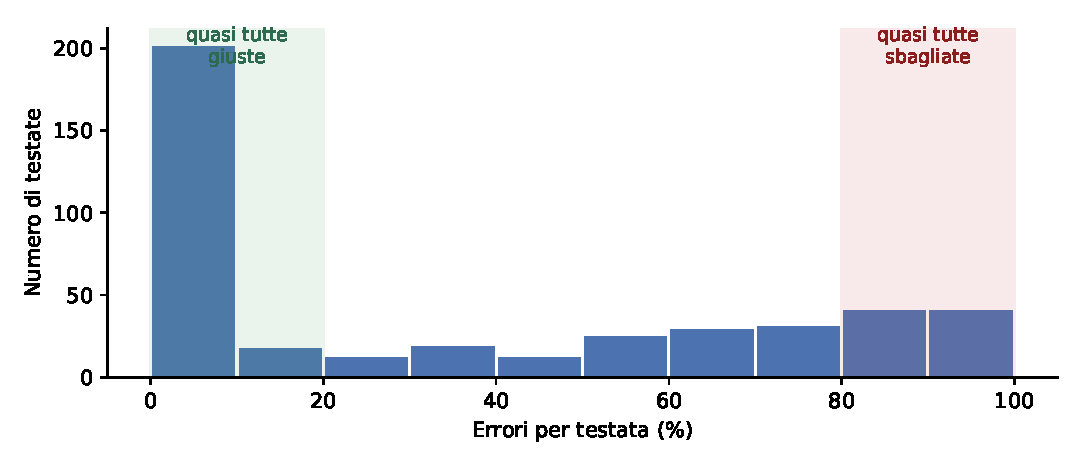
\includegraphics[width=\linewidth]{pub_error_hist.pdf}}
    \end{column}
  \end{columns}
\end{frame}

\begin{frame}{Osservazione di John --- come leggere 0,6}
  \vfill
  \begin{itemize}[<+->]
    \setlength\itemsep{0.8em}
    \item Prova: \hl{rimescoliamo a caso} gli errori tra le testate (tenendo fisso il livello), cos\`i la testata non pu\`o pi\`u contare
    \item In questo mondo ``a caso'' l'ICC viene circa \hl{0,14}
    \item L'abbiamo rifatto 100 volte: non \`e \hl{mai} andato oltre $\sim$0,17
    \item Il nostro \`e \hl{0,6}: pi\`u di 4 volte tanto
    \item Quindi il risultato \hl{non \`e casuale}: gli errori si concentrano davvero in alcune testate
  \end{itemize}
  \vfill
\end{frame}

\begin{frame}{Osservazione di John --- la conclusione}
  \vfill
  \begin{itemize}[<+->]
    \setlength\itemsep{0.9em}
    \item Gli articoli di una testata \hl{non sono prove indipendenti}
    \item Quindi l'unit\`a giusta per il test sono le \hl{439 testate}, non i 19.476 articoli
    \item[] {\small\itshape E vale anche a parit\`a di livello: non \`e solo perch\'e su $l_5$ il modello sbaglia di pi\`u.}
    \item La correzione \`e semplice: fare il test \hl{per testata}
  \end{itemize}
  \vfill
\end{frame}

\begin{frame}{Osservazione di John --- come si fa il test per testata}
  \vfill
  \begin{itemize}[<+->]
    \setlength\itemsep{0.8em}
    \item Per ogni testata, il \hl{voto di maggioranza} dei suoi articoli d\`a \hl{un solo giudizio}
    \item[] {\small\itshape Es.: una testata di livello 1 con 9 articoli: 7 predetti $l_2$, 1 $l_5$, 1 $l_1$ $\rightarrow$ voto $l_2$ $\rightarrow$ testata sbagliata.}
    \item Ogni testata conta \hl{una volta sola}: giusta o sbagliata
    \item Si rif\`a la stessa tabella di prima (orientamento $\times$ giusta/sbagliata), ma con \hl{439 testate} invece di 19.476 articoli
  \end{itemize}
  \vfill
\end{frame}

\begin{frame}{Osservazione di John --- il test per testata: il risultato}
  \begin{columns}[c]
    \begin{column}{0.48\textwidth}
      \begin{itemize}[<+->]
        \setlength\itemsep{0.8em}
        \item $\chi^2$ per testata: \hl{18,8} (contro 1.418 per articolo)
        \item Ancora sopra la soglia di 9,5: il legame \hl{resta}\dots
        \item \dots ma \`e molto meno ``clamoroso''
        \item[] {\small\itshape Esempio con RoBERTa; gli altri modelli danno da 19 a 45.}
      \end{itemize}
    \end{column}
    \begin{column}{0.52\textwidth}
      \visible<2->{%
      \footnotesize
      \begin{center}
      RoBERTa, una riga per orientamento\\[0.3em]
      \begin{tabular}{lrr}
        \toprule
        \textbf{Orientamento} & \textbf{Giuste} & \textbf{Sbagliate} \\
        \midrule
        Far Left       & 9   & 11 \\
        Slightly Left  & 29  & 21 \\
        Non labelled   & 81  & 29 \\
        Slightly Right & 156 & 51 \\
        Far Right      & 28  & 24 \\
        \bottomrule
      \end{tabular}
      \end{center}}
    \end{column}
  \end{columns}
\end{frame}

\begin{frame}{Problema 2 --- cosa dice ChatGPT}
  \vfill
  \begin{itemize}[<+->]
    \setlength\itemsep{0.9em}
    \item Nel paper l'errore \`e calcolato \hl{separatamente per ogni orientamento}
    \item E si afferma che cos\`i \`e ``\hl{indipendente dalla frequenza delle classi}''
    \item In altre parole: calcolarlo separatamente dovrebbe renderlo \hl{non influenzato} da come sono distribuiti i dati
    \item ChatGPT fa notare: \`e vero \hl{solo a met\`a}
  \end{itemize}
  \vfill
\end{frame}

\begin{frame}{Problema 2 --- perch\'e solo a met\`a}
  \vfill
  \begin{itemize}[<+->]
    \setlength\itemsep{0.9em}
    \item Calcolarlo separatamente toglie l'effetto della \hl{dimensione} del gruppo (quanti articoli ha)
    \item Ma \hl{non} toglie l'effetto di \hl{quali livelli} ci sono dentro
    \item E il livello pesa tanto: $l_1$ facile, $l_5$ difficile
    \item Ogni orientamento ha un \hl{mix di livelli diverso}
  \end{itemize}
  \vfill
\end{frame}

\begin{frame}{Problema 2 --- l'esempio}
  \vfill
  \begin{itemize}[<+->]
    \setlength\itemsep{0.9em}
    \item Slightly Right \`e quasi tutto $l_1$ (il livello facile)
    \item Quindi il suo errore basso dipende dal fatto che \`e \hl{pieno di articoli facili}\dots
    \item[] {\small\itshape \dots non dal fatto che il modello ``tratti meglio'' la destra.}
    \item Conclusione: la frase va riscritta --- l'errore per orientamento \hl{dipende ancora} dalla composizione dei livelli
  \end{itemize}
  \vfill
\end{frame}

% ---- Commento di John al Problema 2 ----
\begin{frame}{Problema 2 --- commento di John}
  \vfill
  \begin{itemize}[<+->]
    \setlength\itemsep{0.9em}
    \item ChatGPT d\`a per scontato che i livelli abbiano \hl{difficolt\`a diverse}
    \item Ma questa cosa \hl{non \`e mai dimostrata}
    \item Il modello sbaglia meno su $l_1$ --- ma ``\hl{sbaglia meno}'' non vuol dire ``\hl{\`e pi\`u facile}''
    \item[] {\small\itshape Potrebbe sbagliare meno per tanti altri motivi: orientamento, tema, com'\`e fatto il dataset.}
    \item Non ha senso dire che $l_1$ \`e pi\`u facile di $l_2$ solo perch\'e il modello \hl{sbaglia meno}
  \end{itemize}
  \vfill
\end{frame}

\begin{frame}{Problema 3 --- orientamento e affidabilit\`a sono ``incollati''}
  \vfill
  \begin{itemize}[<+->]
    \setlength\itemsep{0.8em}
    \item Non solo intrecciati: in alcune combinazioni i dati \hl{mancano del tutto}
    \item Nessuna testata far-right \`e in $l_5$; 142 su 207 slightly-right sono in $l_1$
    \item Quando due variabili sono cos\`i sovrapposte, \hl{nessuna analisi} pu\`o separarle del tutto
  \end{itemize}
  \vfill
\end{frame}


\begin{frame}{Problema 4 --- il $\chi^2$ ha bisogno di abbastanza dati}
  \vfill
  \begin{itemize}[<+->]
    \setlength\itemsep{0.9em}
    \item Il $\chi^2$ confronta, in ogni casella, quello che \hl{osserva} con quello che \hl{si aspetterebbe}
    \item Funziona solo se in ogni casella ci sono \hl{abbastanza osservazioni} (regola pratica: almeno $\sim$5 attese)
    \item Con poche testate, alcune caselle sono quasi \hl{vuote}
  \end{itemize}
  \vfill
\end{frame}

\begin{frame}{Problema 4 --- nel nostro caso}
  \begin{columns}[c]
    \begin{column}{0.47\textwidth}
      \begin{itemize}[<+->]
        \setlength\itemsep{0.7em}
        \item Testate divise in 5 orientamenti: \hl{Far Left ne ha solo 20}
        \item Nella casella ``Far Left sbagliate'' ne aspettiamo appena \hl{6,2}: proprio al limite (perch\'e: slide successive)
        \item E guardando orientamento \emph{e} livello insieme, alcune caselle sono \hl{vuote}: nessuna far-right di livello 5, nessuna slightly-left di livello 1
        \item[] {\small\itshape L\`i il $\chi^2$ non ha pi\`u senso.}
      \end{itemize}
    \end{column}
    \begin{column}{0.53\textwidth}
      \visible<2->{%
      \footnotesize
      \begin{center}
      Test per testata, RoBERTa\\[0.3em]
      \begin{tabular}{lrrr}
        \toprule
        & & \multicolumn{2}{c}{\textbf{Sbagliate}} \\
        \cmidrule(lr){3-4}
        \textbf{Orientamento} & \textbf{Testate} & \textbf{osservate} & \textbf{attese} \\
        \midrule
        Far Left       & 20  & 11 & \textbf{6,2} \\
        Slightly Left  & 50  & 21 & 15,5 \\
        Non labelled   & 110 & 29 & 34,1 \\
        Slightly Right & 207 & 51 & 64,1 \\
        Far Right      & 52  & 24 & 16,1 \\
        \bottomrule
      \end{tabular}
      \end{center}}
    \end{column}
  \end{columns}
\end{frame}

\begin{frame}{Problema 4 --- perch\'e servono caselle piene (1)}
  \vfill
  \begin{itemize}[<+->]
    \setlength\itemsep{0.8em}
    \item Il $\chi^2$ somma, casella per casella: $\dfrac{(\text{osservato} - \text{atteso})^2}{\text{atteso}}$
    \item Poi confronta il totale con la soglia di \hl{9,5}: ma quella soglia \`e calcolata supponendo caselle \hl{abbastanza piene}
    \item Con caselle piccole, \hl{una sola testata} pesa moltissimo:
    \item[] casella con 2 attese, ne osservo 4: $\;(4-2)^2/2 = \mathbf{2}$
    \item[] casella con 50 attese, ne osservo 52: $\;(52-50)^2/50 = \mathbf{0{,}08}$
    \item[] {\small\itshape Stessa differenza di 2 testate, peso 25 volte diverso.}
  \end{itemize}
  \vfill
\end{frame}

\begin{frame}{Problema 4 --- perch\'e servono caselle piene (2)}
  \vfill
  \begin{itemize}[<+->]
    \setlength\itemsep{0.8em}
    \item Nel nostro caso (RoBERTa) il $\chi^2$ per testata vale \hl{18,8}
    \item Le sole 20 testate Far Left ne portano \hl{5,4}: quasi un terzo
    \item Se \hl{una} testata Far Left passasse da sbagliata a giusta: $\chi^2$ da 18,8 a \hl{16,9}
    \item Se lo facesse una testata Slightly Right: da 18,8 a 19,5
    \item[] {\small\itshape Il risultato dipende molto da pochissime testate.}
    \item Regola pratica: almeno \hl{5 attese} per casella. Noi ne abbiamo 6,2: appena sopra, \hl{al limite}
  \end{itemize}
  \vfill
\end{frame}


\begin{frame}{Problema 5 --- la MED guarda solo gli errori}
  \vfill
  \begin{itemize}[<+->]
    \setlength\itemsep{1.0em}
    \item La MED misura la direzione dell'errore \hl{solo quando il modello sbaglia}
    \item Non tiene conto di \hl{quanto spesso} sbaglia
  \end{itemize}
  \vfill
\end{frame}

\begin{frame}{Problema 5 --- l'esempio}
  \vfill
  \begin{itemize}[<+->]
    \setlength\itemsep{0.7em}
    \item Gruppo A: sbaglia il \hl{70\%} degli articoli, e quando sbaglia sovrastima di mezzo livello (MED $+0.5$)
    \item Gruppo B: sbaglia il \hl{10\%}, con la stessa MED $+0.5$
    \item Stessa MED, ma l'effetto totale \`e \hl{diversissimo}: A viene spinto in alto 7 volte su 10, B solo 1 su 10
    \item[] {\small\itshape Nel paper gli estremi sbagliano il 60--72\%, i non-labelled il 30\%: confrontare le loro MED inganna.}
    \item Soluzione: riportare anche la direzione media su \hl{tutti} gli articoli, compresi quelli classificati \hl{correttamente} (che contano zero)
  \end{itemize}
  \vfill
\end{frame}

\begin{frame}{Problema 5 --- un'incoerenza nel paper bocciato}
  \vfill
  \begin{itemize}[<+->]
    \setlength\itemsep{0.9em}
    \item La \hl{formula} della MED usa solo gli articoli \hl{sbagliati}
    \item Ma i numeri \hl{per livello} (es.\ $l_5 \approx -1{,}30$) sono calcolati su \hl{tutti} gli articoli
    \item Mentre quelli \hl{per orientamento} (estremi da $+0{,}33$ a $+1{,}00$) solo sugli \hl{errori}
    \item[] {\small\itshape Due definizioni diverse nello stesso paper: nel nuovo va scelta una sola, e dichiarata.}
  \end{itemize}
  \vfill
\end{frame}

\begin{frame}{Problema 6 --- la direzione \`e ``obbligata'' dai bordi}
  \vfill
  \begin{itemize}[<+->]
    \setlength\itemsep{0.8em}
    \item Se una testata \`e in $l_1$ (il pi\`u basso), l'errore pu\`o solo andare \hl{verso l'alto}; se \`e in $l_5$, solo verso il basso
    \item Far-left e far-right stanno quasi tutti nei livelli bassi $\rightarrow$ i loro errori sono ``per forza'' positivi
    \item[] {\small\itshape Quindi la sovrastima degli estremi pu\`o dipendere dalla composizione, non dall'orientamento.}
  \end{itemize}
  \vfill
\end{frame}


% ================================================================
%  CONSIDERAZIONE DI JOHN A CHATGPT (al posto della conclusione di ChatGPT)
% ================================================================
\begin{frame}{Considerazione di John a ChatGPT (1)}
  \vfill
  \begin{itemize}[<+->]
    \setlength\itemsep{0.8em}
    \item L'affidabilit\`a l'abbiamo \hl{stratificata} nei fold (tenuta sotto controllo)
    \item L'orientamento invece \hl{no}: \`e lasciato a caso
    \item E nel dataset orientamento $\times$ livello \`e \hl{sbilanciatissimo}
    \item Alcune combinazioni \hl{non esistono}: nessuna slightly-left di livello 1, nessuna far-right di livello 5
  \end{itemize}
  \vfill
\end{frame}

\begin{frame}{Considerazione di John a ChatGPT (2)}
  \vfill
  \begin{itemize}[<+->]
    \setlength\itemsep{0.8em}
    \item Quando dividiamo in fold, a volte il modello vede \hl{zero} esempi di una combinazione che poi deve indovinare
    \item Es.\ (fold 1): nessun Far Left di livello 1 o 3 in addestramento, ma viene testato proprio su quelli
    \item[] {\small\itshape Naturale che sbagli: non li ha mai visti.}
    \item Quindi parte di questi ``errori politici'' \`e un \hl{artefatto} del dataset e dei fold
  \end{itemize}
  \vfill
\end{frame}

\begin{frame}{Considerazione di John a ChatGPT (3)}
  \vfill
  \begin{itemize}[<+->]
    \setlength\itemsep{0.9em}
    \item Questa analisi del bias \`e \hl{molto specifica}: vale per \emph{questo} dataset, \emph{questi} modelli, \emph{questo} training
    \item Non \`e un risultato generale sul ``comportamento politico'' dei modelli
    \item Se la teniamo, va detto \hl{chiaramente}
    \item[] {\small\itshape \`E un po' un'analisi fine a s\'e stessa.}
  \end{itemize}
  \vfill
\end{frame}

% ---- Considerazione generale di John (non rivolta a ChatGPT) ----
\begin{frame}{Considerazione di John --- che cos'\`e una testata?}
  \begin{alertblock}{Una critica nostra, non a ChatGPT}
    Nel paper una testata coincide con \hl{l'insieme dei suoi articoli}. Ma \`e davvero cos\`i?
  \end{alertblock}
  \vspace{0.6em}
  \begin{itemize}[<+->]
    \setlength\itemsep{0.8em}
    \item Oggi una testata \`e anche le sue \hl{pagine social}, le \hl{newsletter}, i \hl{podcast}, i video
    \item Noi guardiamo solo gli \hl{articoli del sito}: una parte della testata, non la testata intera
    \item[] {\small\itshape Rischiamo di giudicare la testata guardandone solo una parte.}
    \item Nel paper non dovremmo darlo per scontato: va detto chiaramente \hl{che cosa} stiamo giudicando
  \end{itemize}
\end{frame}

% ================================================================
%  FABIO x CLAUDE: solo cio' che e' nuovo rispetto a revisori e ChatGPT
% ================================================================
\begin{frame}{Fabio $\times$ Claude --- cos'\`e}
  \vfill
  \begin{itemize}[<+->]
    \setlength\itemsep{0.9em}
    \item Fabio ha chiesto a Claude tre cose: come usare i modelli grandi, una review del paper, come impostare l'analisi del bias
    \item Il bias l'abbiamo \hl{gi\`a visto}: non ci torniamo
    \item Qui solo le \hl{proposte nuove}: esperimenti, metodi, aggregazione, correzioni
  \end{itemize}
  \vfill
\end{frame}

% ---------------------------------------------------------------- B. baseline e LLM
\begin{frame}{Fabio --- il problema della ``contaminazione''}
  \vfill
  \begin{itemize}[<+->]
    \setlength\itemsep{0.8em}
    \item Domanda di ogni lettore: ``perch\'e non chiedere direttamente a GPT?''
    \item Ma un LLM grande \hl{conosce gi\`a} queste testate: le ha lette in addestramento e ne sa la reputazione
    \item E negli articoli il nome della testata compare spesso (firma, pi\`e di pagina, link)
    \item Quindi GPT potrebbe \hl{ricordare la reputazione} invece di leggere il testo
    \item[] {\small\itshape Come far giudicare un vino ``alla cieca'' lasciando l'etichetta sulla bottiglia.}
  \end{itemize}
  \vfill
\end{frame}

\begin{frame}{Fabio --- l'esperimento: con e senza nomi}
  \vfill
  \begin{itemize}[<+->]
    \setlength\itemsep{0.8em}
    \item Si fa valutare a un LLM lo stesso articolo due volte: \hl{normale} e con nomi, siti e firme \hl{cancellati}
    \item Se senza nomi va molto peggio $\rightarrow$ prima stava \hl{riconoscendo la testata}, non giudicando il testo
    \item Trasforma la domanda ``perch\'e non GPT?'' in un \hl{risultato}
    \item E spiega perch\'e i modelli piccoli addestrati da noi sono lo strumento giusto per \emph{questa} domanda
  \end{itemize}
  \vfill
\end{frame}

\begin{frame}{Fabio --- una baseline semplice: TF-IDF}
  \vfill
  \begin{itemize}[<+->]
    \setlength\itemsep{0.8em}
    \item Oggi confrontiamo i transformer solo con baseline ``stupide'' (classe pi\`u frequente, caso)
    \item Fabio: aggiungere un modello \hl{semplice ma serio}, senza reti neurali
    \item \hl{TF-IDF}: conta le parole di ogni articolo, dando pi\`u peso a quelle rare e distintive; sopra, una regressione logistica
    \item[] {\small\itshape Se un ``contatore di parole'' arriva vicino ai transformer, i transformer non stanno aggiungendo molto.}
    \item Costa pochissimo da fare
  \end{itemize}
  \vfill
\end{frame}

% ---------------------------------------------------------------- C. nuovi metodi
\begin{frame}{Fabio --- LLM come estrattore di segnali: l'idea}
  \vfill
  \begin{itemize}[<+->]
    \setlength\itemsep{0.8em}
    \item Invece di chiedere all'LLM ``\`e affidabile?'', gli si chiede un \hl{voto su segnali precisi}
    \item[] {\small\itshape Sensazionalismo, fonti citate, toni prudenti, opinione o cronaca, titolo acchiappa-clic, presenza di rettifiche\dots}
    \item Ogni articolo diventa una \hl{lista di voti}
    \item[] {\small\itshape Es.: sensazionalismo 8/10, fonti citate 2/10, opinione 9/10, \dots}
    \item Poi un classificatore semplice impara \hl{quali segnali contano}
  \end{itemize}
  \vfill
\end{frame}

\begin{frame}{Fabio --- LLM come estrattore di segnali: perch\'e}
  \vfill
  \begin{itemize}[<+->]
    \setlength\itemsep{0.8em}
    \item \hl{Costa poco}: una chiamata all'LLM per articolo ($\sim$20.000 in tutto)
    \item \hl{Si capisce}: sappiamo \emph{quali} segnali distinguono una testata affidabile
    \item Aggregare \`e naturale: il profilo di una testata \`e la \hl{media} dei voti dei suoi articoli
    \item Per Fabio \`e la proposta con il miglior rapporto novit\`a/fatica, insieme all'esperimento con e senza nomi
  \end{itemize}
  \vfill
\end{frame}

\begin{frame}{Fabio --- multiple-instance learning: l'idea}
  \vfill
  \begin{itemize}[<+->]
    \setlength\itemsep{0.8em}
    \item Oggi: classifichiamo \hl{ogni articolo}, poi \hl{votiamo}
    \item Ma l'etichetta vera \`e della \hl{testata}, non del singolo articolo
    \item Idea: addestrare il modello direttamente su ``\hl{sacchetti}'' di articoli: tutti quelli di una testata insieme, con l'etichetta della testata
    \item[] {\small\itshape Come giudicare un ristorante leggendo tutte le recensioni insieme, invece di dare un voto a ciascuna e fare la maggioranza.}
  \end{itemize}
  \vfill
\end{frame}

\begin{frame}{Fabio --- multiple-instance learning: come}
  \vfill
  \begin{itemize}[<+->]
    \setlength\itemsep{0.8em}
    \item Ogni articolo viene trasformato una volta in un \hl{embedding}: una lista di numeri che ne riassume il significato
    \item Il modello impara a combinare gli embedding di una testata (media, o pesando di pi\`u gli articoli pi\`u utili)
    \item 439 testate sono poche: si creano tanti sacchetti \hl{a caso} da 10--20 articoli della stessa testata $\rightarrow$ migliaia di esempi
    \item In pi\`u d\`a una \hl{misura di confidenza} sul giudizio della testata
  \end{itemize}
  \vfill
\end{frame}

\begin{frame}{Fabio --- modelli pi\`u recenti e altre idee}
  \vfill
  \begin{itemize}[<+->]
    \setlength\itemsep{0.7em}
    \item BERT e Llama~3 sembrano ``datati'': stessa ricetta con modelli attuali (\hl{ModernBERT}, \hl{DeBERTa-v3}, piccoli decoder recenti)
    \item[] {\small\itshape Quasi solo estetica, ma toglie un appiglio ai revisori.}
    \item \hl{Pulizia delle etichette}: un LLM segnala gli articoli atipici per la loro testata e si d\`a loro meno peso
    \item \hl{Agente}: visita la testata, legge le pagine ``chi siamo'', propriet\`a, rettifiche, e valuta i 9 criteri di NewsGuard
    \item[] {\small\itshape \`E un altro task (non solo testo): lavoro futuro.}
  \end{itemize}
  \vfill
\end{frame}

\begin{frame}{Fabio --- la distillazione: cos'\`e}
  \vfill
  \begin{itemize}[<+->]
    \setlength\itemsep{0.8em}
    \item Un modello \hl{grande} (``insegnante'', es.\ un LLM) serve ad addestrare un modello \hl{piccolo} (``studente'')
    \item L'insegnante legge gli articoli e d\`a le sue risposte; lo studente impara a \hl{imitarle}
    \item[] {\small\itshape Come uno studente che impara dagli appunti del professore, non solo dal libro.}
    \item Per Fabio, nella forma base serve a poco: le etichette giuste (NewsGuard) le abbiamo gi\`a, e l'insegnante porterebbe dentro la sua \hl{contaminazione} (riconosce le testate)
  \end{itemize}
  \vfill
\end{frame}

\begin{frame}{Fabio --- la distillazione: come andrebbe fatta}
  \vfill
  \begin{enumerate}[<+->]
    \setlength\itemsep{0.8em}
    \item Per ogni articolo l'LLM scrive una \hl{breve spiegazione}: perch\'e sembra affidabile o no
    \item[] {\small\itshape Es.: ``titolo sensazionalistico, nessuna fonte citata, tono da opinione''.}
    \item Il modello piccolo viene addestrato a dare \hl{l'etichetta NewsGuard} \emph{e} a riprodurre la \hl{spiegazione}
    \item Cos\`i impara \emph{su cosa} guardare, non solo il risultato $\rightarrow$ gli servono \hl{meno dati}
  \end{enumerate}
  \vspace{0.6em}
  \visible<5->{\small\itshape Per Fabio: guadagno incerto e parecchio lavoro, non prioritaria.}
  \vfill
\end{frame}

% ---------------------------------------------------------------- D. aggregazione
\begin{frame}{Fabio --- confrontare modi di aggregare}
  \vfill
  \begin{itemize}[<+->]
    \setlength\itemsep{0.8em}
    \item Oggi usiamo un solo modo: il \hl{voto di maggioranza}
    \item Alternative: \hl{media} dei livelli, \hl{mediana}, media delle \hl{probabilit\`a}
    \item Esempio, 10 articoli: 4 dicono $l_2$, 3 dicono $l_3$, 3 dicono $l_4$
    \item[] Maggioranza: $l_2$ \qquad Media: $(4{\cdot}2+3{\cdot}3+3{\cdot}4)/10 = 2{,}9 \rightarrow l_3$
    \item Risposte \hl{diverse}: vale la pena confrontarle
  \end{itemize}
  \vfill
\end{frame}

\begin{frame}{Fabio --- quanti articoli servono?}
  \vfill
  \begin{itemize}[<+->]
    \setlength\itemsep{0.8em}
    \item Domanda pratica: per giudicare una testata \hl{nuova}, quanti articoli mi servono?
    \item La curva: accuratezza sulla testata usando 5, 10, 20, 50\dots\ articoli
    \item Con fino a 200 articoli il voto \`e probabilmente gi\`a ``saturo'': la domanda interessante \`e \hl{con pochi}
    \item[] {\small\itshape \`E l'informazione pi\`u utile per chi volesse usare il sistema davvero.}
  \end{itemize}
  \vfill
\end{frame}

% ---------------------------------------------------------------- E. altri punti nuovi
\begin{frame}{Fabio --- l'early stopping: cos'\`e}
  \vfill
  \begin{itemize}[<+->]
    \setlength\itemsep{0.8em}
    \item Il modello si addestra in pi\`u ``giri'' sugli stessi dati (le \hl{epoche})
    \item Dopo un po' comincia a \hl{imparare a memoria} gli esempi e peggiora sui dati nuovi
    \item Early stopping: dopo ogni giro misuro l'errore su dati \hl{messi da parte} (``validation'') e tengo la versione migliore
    \item[] {\small\begin{tabular}{lccccc}
      \toprule
      \textbf{Giro} & 1 & 2 & 3 & 4 & 5 \\
      \textbf{Errore sulla validation} & 0,60 & 0,50 & 0,46 & \hl{0,44} & 0,47 \\
      \bottomrule
    \end{tabular}}
    \item[] {\small\itshape Tengo il giro 4: dopo, il modello peggiora (come Llama nel paper, minimo al giro 4).}
  \end{itemize}
  \vfill
\end{frame}

\begin{frame}{Fabio --- l'early stopping: il rischio}
  \vfill
  \begin{itemize}[<+->]
    \setlength\itemsep{0.8em}
    \item I dati di validation devono essere \hl{diversi} da quelli di test
    \item Se scegliessi il giro migliore guardando il \hl{test}, sceglierei la versione che \emph{per caso} va meglio proprio sul test
    \item[] {\small\itshape Come scegliere quale compito consegnare dopo aver visto le soluzioni: il voto sembra pi\`u alto di quello che vali.}
    \item Il risultato riportato sarebbe \hl{gonfiato}
  \end{itemize}
  \vfill
\end{frame}

\begin{frame}{Fabio --- l'early stopping: nel nostro caso}
  \vfill
  \begin{itemize}[<+->]
    \setlength\itemsep{0.8em}
    \item Nel paper: ``early stopping che salva il modello con la validation loss minima'', senza dire \hl{su quali dati}
    \item Dal codice: lo usa \hl{solo Llama}, su un 10\% degli articoli di \hl{training}; gli altri modelli fanno un numero fisso di giri
    \item Quindi nessuna contaminazione, ma \hl{va scritto} chiaramente
  \end{itemize}
  \vfill
\end{frame}

\begin{frame}{Fabio --- tema e periodo}
  \vfill
  \begin{itemize}[<+->]
    \setlength\itemsep{0.8em}
    \item Gli articoli sono presi dalle homepage in un \hl{periodo breve}: ogni testata porta i \hl{temi del momento}
    \item Se tema e affidabilit\`a vanno insieme, il modello potrebbe imparare il \hl{tema}, non l'affidabilit\`a
    \item[] {\small\itshape Es.: se quella settimana le testate inaffidabili parlano tutte dello stesso argomento, basta riconoscere l'argomento.}
    \item Controllo: classificare il tema degli articoli e vedere se \`e legato al livello
  \end{itemize}
  \vfill
\end{frame}

\begin{frame}{Fabio --- la classe $l_5$ e l'ordine dei livelli}
  \vfill
  \begin{itemize}[<+->]
    \setlength\itemsep{0.8em}
    \item $l_5$ = punteggio \hl{esattamente 100}: classe piccola e quasi impossibile da distinguere da $l_4$
    \item Proposta: \hl{unire} $l_4$ e $l_5$, o riportare anche i risultati a 4 classi
    \item I livelli sono \hl{ordinati}, ma il modello \`e addestrato come se fossero categorie slegate
    \item[] {\small\itshape In addestramento confondere $l_5$ con $l_4$ costa quanto confonderlo con $l_1$: va almeno detto come limite.}
  \end{itemize}
  \vfill
\end{frame}

\begin{frame}{Fabio --- correzioni di scrittura (verificate)}
  \vfill
  \small
  \begin{itemize}[<+->]
    \setlength\itemsep{0.55em}
    \item Bibliografia doppia: [4] = [15] (Przyby\l{}a \& Soto), [5] = [20] (Srba et al.)
    \item {[30]} cita ``Mixtral of Experts'' per Mistral 24B: \`e un modello diverso
    \item Rinvii sbagliati: ``In V-B we instantiate Agg'' (\`e V-E), ``Section IV-0c''
    \item Tabella II: BERT 58,27\%, mentre il testo dice ``around 0.60'' (dato complessivo contro media sui fold)
    \item Il contributo 4 \`e un \hl{risultato}, non un contributo; i contributi 1--2 si sovrappongono a Burdisso et al.\ [7]
    \item Dire chiaramente se il dataset \`e \hl{rilasciabile} (etichette NewsGuard proprietarie)
  \end{itemize}
  \vfill
\end{frame}

% ---------------------------------------------------------------- esperimenti di John
\divider{Esperimenti di John}{dal dataset dello scraping a un dataset pulito}

\begin{frame}{Esperimenti --- da dove partiamo}
  \vfill
  \begin{itemize}[<+->]
    \setlength\itemsep{0.8em}
    \item Il dataset dello scraping, \hl{cos\`i com'\`e}: scraping + filtro della lingua, 439 testate, 19.476 articoli
    \item L'ordine logico: prima si \hl{controllano e puliscono i dati}, poi si classifica
    \item Regola per la pulizia: \hl{nessun classificatore e nessuna etichetta}
    \item[] {\small\itshape Le etichette NewsGuard si guardano solo alla fine, per descrivere e valutare: cos\`i nessuno pu\`o dire che abbiamo pulito i dati in base ai risultati.}
    \item Tutto in notebook Jupyter, eseguibili da capo: cartella \texttt{Code/WebScience2027}
  \end{itemize}
  \vfill
\end{frame}

\begin{frame}{Esperimenti --- che cosa cerchiamo: le testate ``parenti''}
  \vfill
  \begin{itemize}[<+->]
    \setlength\itemsep{0.8em}
    \item Molte testate \hl{non sono indipendenti}: reti di siti con lo stesso proprietario, giornali della stessa catena, articoli ripresi da pi\`u testate
    \item Due testate sono \hl{parenti} se pubblicano lo \hl{stesso testo}
    \item Il rischio: una sorella nel training e una nel test
    \item[] {\small\itshape Il classificatore riconosce il testo gi\`a visto, invece di giudicare l'affidabilit\`a.}
    \item Per trovarle basta il \hl{testo}: non serve nessun modello
  \end{itemize}
  \vfill
\end{frame}

\begin{frame}{Passo 1 --- articoli quasi uguali (1)}
  \vfill
  \begin{itemize}[<+->]
    \setlength\itemsep{0.7em}
    \item Prima si \hl{normalizza} il testo: minuscole, niente punteggiatura, numeri sostituiti da \#
    \item[] {\small\itshape ``In 2024, Cook County collected \$12.5 million'' $\rightarrow$ ``in \# cook county collected \# \# million''}
    \item Ogni articolo si spezza in \hl{pezzetti di 5 parole} consecutive
    \item Due articoli sono \hl{quasi uguali} se condividono almeno \hl{met\`a} dei pezzetti
    \item[] {\small\itshape Somiglianza = pezzetti in comune / pezzetti totali dei due articoli (Jaccard).}
    \item Le coppie da confrontare sarebbero quasi 200 milioni: \hl{MinHash} riassume ogni articolo in un'impronta e propone solo le coppie candidate
  \end{itemize}
  \vfill
\end{frame}

\begin{frame}{Passo 1 --- articoli quasi uguali (2)}
  \begin{columns}[c]
    \begin{column}{0.48\textwidth}
      \begin{itemize}[<+->]
        \setlength\itemsep{0.8em}
        \item \hl{1.557 articoli} hanno un testo \hl{identico} su un'altra testata
        \item Il \hl{24\%} degli articoli ha una copia quasi uguale su un'altra testata
        \item Esempio: lo stesso articolo sui prezzi della benzina su due siti diversi, cambia solo la contea
      \end{itemize}
    \end{column}
    \begin{column}{0.52\textwidth}
      \visible<3->{%
      \scriptsize
      \begin{block}{\scriptsize Testata A}
        ``There was a single gas station in cities across \textbf{Phillips County} selling regular gas at the price of \$3.09 per gallon in the week ending Mar.~15, according to customer reports submitted to GasBuddy.com''
      \end{block}
      \begin{block}{\scriptsize Testata B}
        ``There was a single gas station in cities across \textbf{Escambia County} selling regular gas at the lowest price of \$2.65 per gallon in the week ending Mar.~15, according to customer reports submitted to GasBuddy.com''
      \end{block}}
    \end{column}
  \end{columns}
\end{frame}

\begin{frame}{Passo 2 --- dai legami ai gruppi}
  \vfill
  \begin{itemize}[<+->]
    \setlength\itemsep{0.8em}
    \item Due testate sono \hl{collegate} se hanno \hl{almeno 2 articoli} quasi uguali in comune
    \item[] {\small\itshape Una sola copia pu\`o essere una notizia ripresa una volta; due o pi\`u indicano un rapporto stabile.}
    \item Un \hl{gruppo} = testate collegate anche indirettamente (A--B e B--C: A, B e C insieme)
    \item Risultato: \hl{10 gruppi} con \hl{236 testate}; le altre \hl{203} sono indipendenti
    \item Il gruppo pi\`u grande ha \hl{131 testate}
  \end{itemize}
  \vfill
\end{frame}

\begin{frame}{Passo 2 --- verifica con il proprietario}
  \vfill
  \begin{itemize}[<+->]
    \setlength\itemsep{0.7em}
    \item NewsGuard riporta il \hl{proprietario} di ogni sito: non l'abbiamo usato per fare i gruppi, solo per \hl{controllarli}
    \item Per ogni testata:
    \item[] -- \hl{precisione}: tra le testate del suo gruppo, quante hanno lo stesso proprietario
    \item[] -- \hl{richiamo}: tra le testate con lo stesso proprietario, quante sono nel suo gruppo
    \item Risultato: precisione \hl{0,93}, richiamo \hl{0,87}
    \item[] {\small\itshape Quasi tutti i gruppi sono davvero ``di famiglia''. Quello che manca sono siti dello stesso proprietario che non condividono testo: per il classificatore sono testate diverse.}
  \end{itemize}
  \vfill
\end{frame}

\begin{frame}{Passo 2 --- e se cambiamo le soglie?}
  \begin{itemize}
    \item Le soglie (2 articoli in comune, somiglianza 0,5) sono fissate \hl{prima}; qui le facciamo variare
  \end{itemize}
  \vspace{0.5em}
  \visible<2->{%
  \centering\small
  \begin{tabular}{crrrr}
    \toprule
    \textbf{Articoli in comune} & \textbf{Gruppi} & \textbf{Testate nei gruppi} & \textbf{Precisione} & \textbf{Richiamo} \\
    \midrule
    almeno 1 & 7 & 264 & 0,79 & 0,91 \\
    \textbf{almeno 2} & \textbf{10} & \textbf{236} & \textbf{0,93} & \textbf{0,87} \\
    almeno 3 & 13 & 215 & 0,96 & 0,80 \\
    almeno 5 & 20 & 205 & 0,98 & 0,77 \\
    \bottomrule
  \end{tabular}\par}
  \vspace{0.8em}
  \begin{itemize}
    \item<3-> Il quadro non cambia: il gruppo pi\`u grande resta di 131 testate, i numeri si spostano poco
  \end{itemize}
\end{frame}

\begin{frame}{Passo 3 --- la pulizia in 4 regole}
  \vfill
  \begin{enumerate}[<+->]
    \setlength\itemsep{0.8em}
    \item \hl{Una sola copia} per articolo: se lo stesso articolo compare su pi\`u testate, se ne tiene una (a caso, seed 42)
    \item \hl{Niente copie tra gruppi diversi}: le poche copie isolate rimaste si tolgono
    \item Via i \hl{paragrafi condivisi}: un paragrafo identico in almeno due testate non \`e testo originale dell'articolo
    \item Via gli articoli rimasti con \hl{100 parole o meno} (la stessa soglia dello scraping)
  \end{enumerate}
  \vspace{0.5em}
  \visible<5->{\small\itshape L'ordine conta: togliendo prima i paragrafi, un articolo ripreso per intero sparirebbe da entrambe le testate.}
  \vfill
\end{frame}

\begin{frame}{Regola 1 --- che cosa vuol dire ``lo stesso articolo''}
  \begin{itemize}[<+->]
    \setlength\itemsep{0.6em}
    \item Somiglianza \hl{almeno 0,9}: lo stesso testo con poche parole cambiate (un pezzo ripreso, o cambia solo il nome della contea)
    \item Tra 0,5 e 0,9: articoli che condividono solo \hl{parti} di testo; restano, le parti comuni spariscono con la regola 3
    \item Perch\'e non pi\`u in basso: gli articoli simili si \hl{uniscono a catena} (A simile a B, B simile a C\dots)
  \end{itemize}
  \vspace{0.4em}
  \visible<3->{%
  \centering\small
  \begin{tabular}{crrr}
    \toprule
    \textbf{Somiglianza minima} & \textbf{Famiglie} & \textbf{Famiglia pi\`u grande} & \textbf{Articoli tolti} \\
    \midrule
    0,7 & 736 & 1.680 & 3.671 \\
    0,8 & 709 & 1.672 & 3.361 \\
    \textbf{0,9} & \textbf{733} & \textbf{52} & \textbf{1.835} \\
    0,95 & 649 & 19 & 1.085 \\
    \bottomrule
  \end{tabular}\par}
\end{frame}

\begin{frame}{Regole 2--4 --- che cosa si toglie}
  \vfill
  \begin{itemize}[<+->]
    \setlength\itemsep{0.7em}
    \item Regola 1: \hl{1.835} copie tolte
    \item Regola 2: \hl{23} coppie tra gruppi diversi, \hl{46} articoli tolti
    \item Regola 3: tolti i paragrafi condivisi, il \hl{5,5\%} delle parole
    \item[] {\small\itshape Es.: la didascalia fissa di una foto, la nota ``the data in this article comes from\dots'', il testo fisso sui prezzi della benzina, ognuno su oltre 100 testate.}
    \item Regola 4: \hl{1.325} articoli rimasti troppo corti
    \item Restano \hl{16.270 articoli} di \hl{436 testate}
  \end{itemize}
  \vfill
\end{frame}

\begin{frame}{La pulizia --- tre controlli}
  \vfill
  \begin{itemize}[<+->]
    \setlength\itemsep{0.8em}
    \item Le testate \hl{indipendenti} restano quasi intatte: tengono il \hl{99,6\%} degli articoli
    \item Le testate \hl{nei gruppi} tengono il \hl{68\%}; il gruppo da 131 testate il \hl{48\%}
    \item[] {\small\itshape La pulizia tocca solo dove c'era testo copiato.}
    \item Rifatta da capo la ricerca degli articoli quasi uguali sul testo pulito: tra gruppi diversi restano \hl{0 coppie} (prima erano 1,45 milioni in tutto)
    \item[] {\small\itshape Dentro uno stesso gruppo ne restano: non fanno danno, perch\'e un gruppo star\`a tutto in un fold.}
  \end{itemize}
  \vfill
\end{frame}

\begin{frame}{Tre versioni del dataset}
  \vfill
  \begin{itemize}[<+->]
    \setlength\itemsep{0.8em}
    \item Una testata con pochissimi articoli d\`a un voto di maggioranza poco affidabile
    \item Tre versioni:
    \item[] -- \hl{min0}: tutte le testate rimaste (436)
    \item[] -- \hl{min10}: solo testate con almeno 10 articoli (365)
    \item[] -- \hl{min20}: solo testate con almeno 20 articoli (246)
    \item Da qui in poi guardiamo i \hl{livelli NewsGuard}, solo per descrivere: la pulizia \`e gi\`a fatta
  \end{itemize}
  \vfill
\end{frame}

\begin{frame}{Tre versioni del dataset --- la composizione}
  \centering
  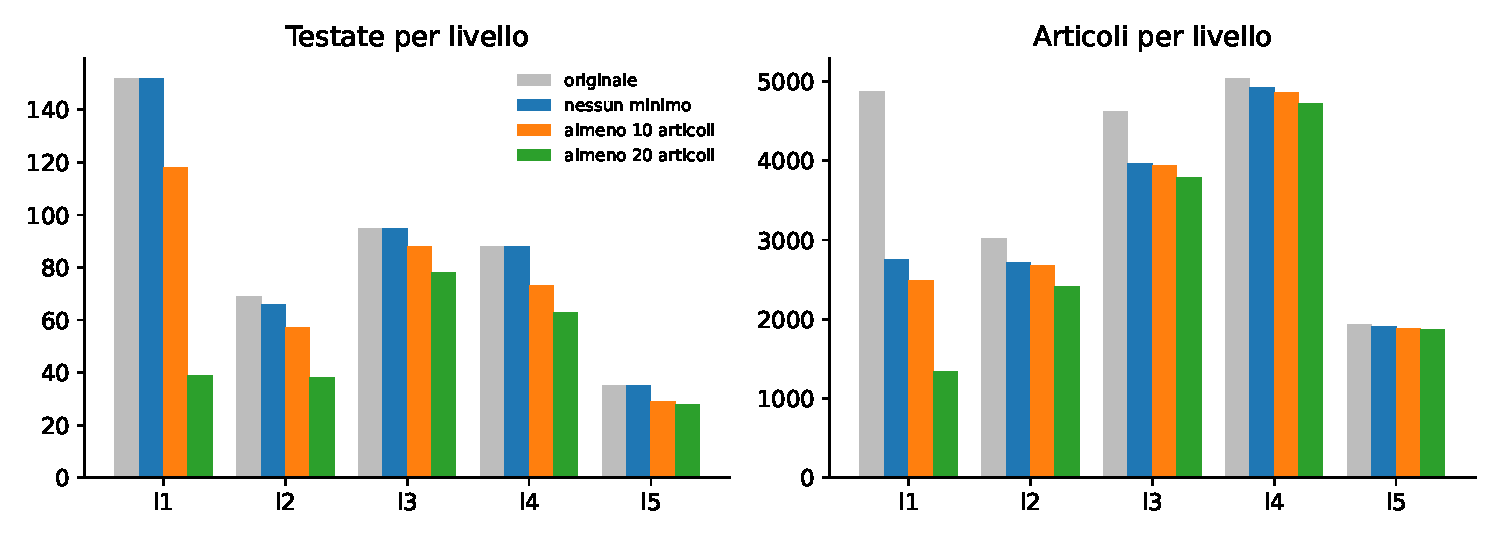
\includegraphics[width=0.95\textwidth]{fig_composizione_versioni.pdf}\\[0.3em]
  \begin{itemize}[<+->]
    \item[] \small $l_1$ \`e il livello pi\`u colpito: tanti siti della rete con pochi articoli originali. Con almeno 20 articoli restano \hl{39 testate $l_1$ su 152}.
  \end{itemize}
\end{frame}

\begin{frame}{Tre versioni del dataset --- i numeri}
  \centering\small
  \begin{tabular}{l rr rr rr rr}
    \toprule
    & \multicolumn{2}{c}{\textbf{Originale}} & \multicolumn{2}{c}{\textbf{min0}} & \multicolumn{2}{c}{\textbf{min10}} & \multicolumn{2}{c}{\textbf{min20}} \\
    \cmidrule(lr){2-3}\cmidrule(lr){4-5}\cmidrule(lr){6-7}\cmidrule(lr){8-9}
    & testate & articoli & testate & articoli & testate & articoli & testate & articoli \\
    \midrule
    $l_1$ & 152 & 4.871 & 152 & 2.758 & 118 & 2.494 & 39 & 1.345 \\
    $l_2$ & 69 & 3.016 & 66 & 2.716 & 57 & 2.678 & 38 & 2.414 \\
    $l_3$ & 95 & 4.620 & 95 & 3.966 & 88 & 3.943 & 78 & 3.788 \\
    $l_4$ & 88 & 5.041 & 88 & 4.924 & 73 & 4.865 & 63 & 4.727 \\
    $l_5$ & 35 & 1.928 & 35 & 1.906 & 29 & 1.882 & 28 & 1.867 \\
    \midrule
    totale & 439 & 19.476 & 436 & 16.270 & 365 & 15.862 & 246 & 14.141 \\
    \bottomrule
  \end{tabular}
\end{frame}

\begin{frame}{Classificazione --- il classificatore a feature}
  \vfill
  \begin{itemize}[<+->]
    \setlength\itemsep{0.8em}
    \item Ogni articolo diventa un \hl{elenco di parole} (e coppie di parole), ciascuna con un peso: TF-IDF
    \item[] {\small\itshape Peso alto = parola frequente in quell'articolo ma rara negli altri.}
    \item Una \hl{regressione logistica} impara quali parole spingono verso ciascun livello
    \item Per la testata: \hl{voto di maggioranza} dei suoi articoli, come nel paper
    \item Metriche come nel paper: accuratezza, F1 macro, tolerant accuracy
  \end{itemize}
  \vfill
\end{frame}

\begin{frame}{Classificazione --- due modi di fare i fold}
  \vfill
  \begin{itemize}[<+->]
    \setlength\itemsep{0.8em}
    \item \hl{Fold per testata} (come nel paper): ogni testata sta in un solo fold, ma le sorelle possono finire in fold diversi
    \item \hl{Fold per gruppo}: ogni gruppo di testate parenti sta tutto in un fold
    \item[] {\small\itshape Nessuna testata ha sorelle nel training: \`e il protocollo che proponiamo.}
    \item I fold sono salvati su file: \hl{BERT usa esattamente gli stessi}
  \end{itemize}
  \vfill
\end{frame}

\begin{frame}{Classificazione --- i risultati}
  \begin{columns}[c]
    \begin{column}{0.55\textwidth}
      \centering
      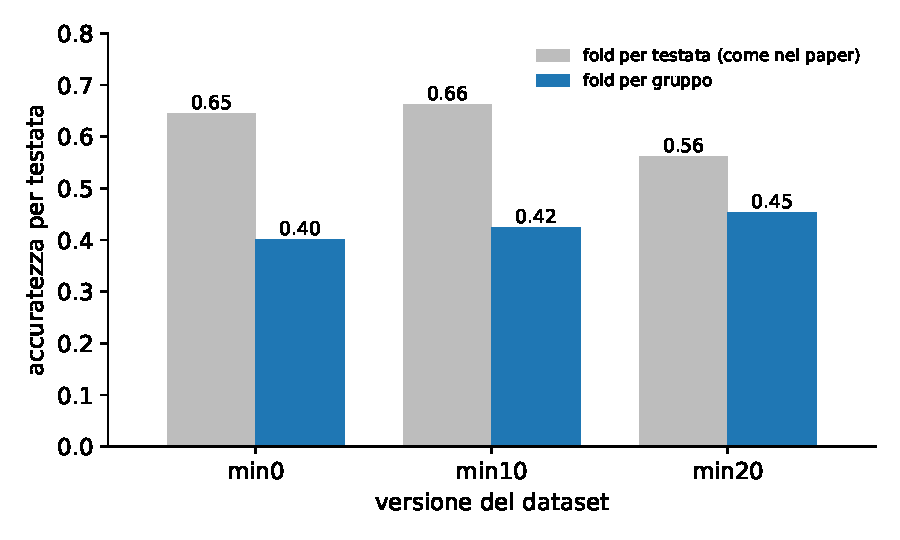
\includegraphics[width=\textwidth]{fig_accuratezza_fold.pdf}
    \end{column}
    \begin{column}{0.45\textwidth}
      \begin{itemize}[<+->]
        \setlength\itemsep{0.7em}
        \item Accuratezza \hl{per testata}, media sui 5 fold
        \item Con i fold del paper: \hl{0,65} (min0)
        \item Con i fold per gruppo: \hl{0,40} (min0)
        \item[] {\small\itshape Sul dataset originale, con i fold del paper, era 0,68.}
      \end{itemize}
    \end{column}
  \end{columns}
\end{frame}

\begin{frame}{Classificazione --- tutte le metriche (per testata)}
  \centering\small
  \begin{tabular}{ll cccc}
    \toprule
    \textbf{Versione} & \textbf{Fold} & \textbf{Accuratezza} & \textbf{F1 macro} & \textbf{Tolerant 0,5} & \textbf{Tolerant 1} \\
    \midrule
    min0 & per testata & 0,65 & 0,53 & 0,75 & 0,85 \\
         & \textbf{per gruppo} & \textbf{0,40} & \textbf{0,33} & \textbf{0,53} & \textbf{0,67} \\
    \midrule
    min10 & per testata & 0,66 & 0,57 & 0,76 & 0,86 \\
          & \textbf{per gruppo} & \textbf{0,42} & \textbf{0,37} & \textbf{0,56} & \textbf{0,69} \\
    \midrule
    min20 & per testata & 0,56 & 0,50 & 0,69 & 0,81 \\
          & \textbf{per gruppo} & \textbf{0,45} & \textbf{0,36} & \textbf{0,59} & \textbf{0,72} \\
    \bottomrule
  \end{tabular}\\[0.8em]
  \raggedright\small\itshape Le tre versioni hanno testate diverse: si confrontano le righe dentro la stessa versione, non tra versioni.
\end{frame}

\begin{frame}{Classificazione --- che cosa ne ricaviamo}
  \vfill
  \begin{itemize}[<+->]
    \setlength\itemsep{0.8em}
    \item \hl{Pulire il testo da solo cambia poco}: con i fold del paper da 0,68 a 0,65
    \item Quello che conta \`e \hl{come si dividono i fold}: con i fold per gruppo si scende a 0,40
    \item[] {\small\itshape Una parte importante del risultato del paper veniva dal riconoscere le testate sorelle (e in parte dalla rete $l_1$, vedi slide successiva).}
    \item Il risultato con i fold per gruppo \`e quello che un modello fa davvero su una testata \hl{nuova}
  \end{itemize}
  \vfill
\end{frame}

\begin{frame}{Classificazione --- livello per livello (min0, fold per gruppo)}
  \begin{columns}[c]
    \begin{column}{0.48\textwidth}
      \centering\small
      Accuratezza per testata (n.\ testate)\\[0.3em]
      \begin{tabular}{lcc}
        \toprule
        & \textbf{Indipendenti} & \textbf{Nei gruppi} \\
        \midrule
        $l_1$ & 0,11 (18) & 0,01 (134) \\
        $l_2$ & 0,64 (42) & 0,54 (24) \\
        $l_3$ & 0,26 (39) & 0,88 (56) \\
        $l_4$ & 0,57 (72) & 0,25 (16) \\
        $l_5$ & 0,12 (32) & 0,00 (3) \\
        \midrule
        tutte & 0,41 (203) & 0,29 (233) \\
        \bottomrule
      \end{tabular}
    \end{column}
    \begin{column}{0.52\textwidth}
      \begin{itemize}[<+->]
        \setlength\itemsep{0.6em}
        \item Il gruppo da 131 siti $l_1$, mai visto nel training: \hl{127 su 131} classificati $l_3$
        \item[] {\small\itshape Tolto il testo fisso, quei pezzi sembrano notizie locali.}
        \item Quando \`e nel test, nel training restano solo \hl{21 testate $l_1$}
        \item Il gruppo di giornali $l_3$ tiene (\hl{0,88}) anche senza sorelle nel training
      \end{itemize}
    \end{column}
  \end{columns}
\end{frame}

\begin{frame}{Un controllo sul dataset originale}
  \begin{columns}[c]
    \begin{column}{0.55\textwidth}
      \centering
      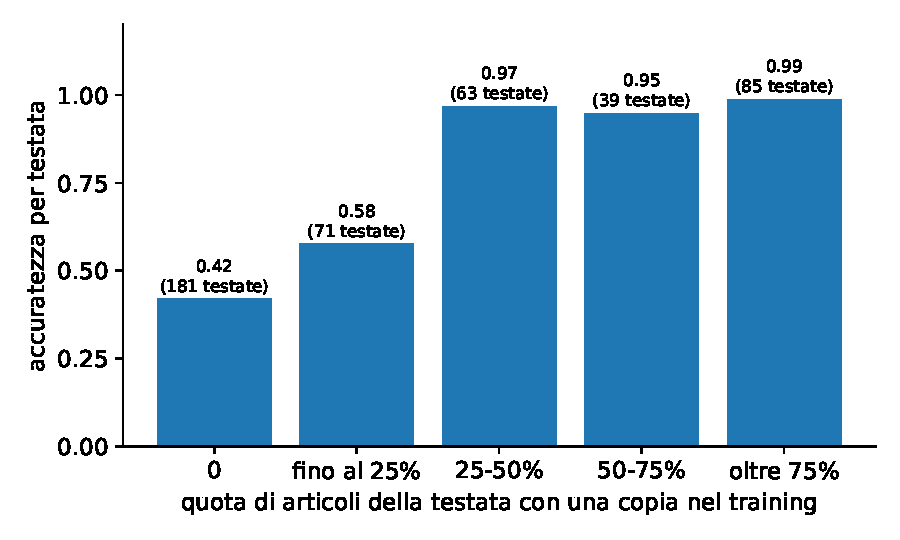
\includegraphics[width=\textwidth]{fig_parentela.pdf}
    \end{column}
    \begin{column}{0.45\textwidth}
      \begin{itemize}[<+->]
        \setlength\itemsep{0.6em}
        \item Dataset \hl{non pulito}, fold del paper
        \item Per ogni testata del test: quota dei suoi articoli con una \hl{copia nel training}
        \item Nessuna copia: accuratezza \hl{0,42}
        \item Oltre il 25\% di copie: \hl{0,95--0,99}
        \item[] {\small\itshape L'accuratezza alta viene quasi tutta dalle testate con copie dei loro articoli nel training.}
      \end{itemize}
    \end{column}
  \end{columns}
\end{frame}

\begin{frame}{BERT --- come l'abbiamo addestrato}
  \vfill
  \begin{itemize}[<+->]
    \setlength\itemsep{0.8em}
    \item Stesse impostazioni del paper: bert-base-uncased, 256 token, 5 epoche, batch 32, learning rate 2e-5
    \item Stessi dati (min0) e \hl{stessi fold per gruppo} del classificatore a feature
    \item Addestramento sul server del gruppo (GPU V100S): circa 14 minuti per fold, 73 minuti in tutto
    \item Domanda: sulle testate \hl{nuove}, BERT fa meglio delle parole?
  \end{itemize}
  \vfill
\end{frame}

\begin{frame}{BERT --- i risultati}
  \centering\small
  min0, fold per gruppo, media sui 5 fold\\[0.4em]
  \begin{tabular}{ll cccc}
    \toprule
    \textbf{Valutazione} & \textbf{Modello} & \textbf{Accuratezza} & \textbf{F1 macro} & \textbf{Tolerant 0,5} & \textbf{Tolerant 1} \\
    \midrule
    per testata  & TF-IDF + LR & 0,40 & 0,33 & 0,53 & 0,67 \\
                 & BERT        & 0,40 & 0,33 & 0,56 & 0,73 \\
    \midrule
    per articolo & TF-IDF + LR & 0,39 & 0,31 & 0,54 & 0,69 \\
                 & BERT        & 0,36 & 0,29 & 0,53 & 0,70 \\
    \bottomrule
  \end{tabular}
  \raggedright
  \begin{itemize}[<+->]
    \setlength\itemsep{0.6em}
    \item<2-> Sulle testate nuove BERT \hl{non fa meglio} del classificatore a feature: 0,40 contro 0,40
    \item<3-> Con i fold del paper, sul dataset originale, BERT arrivava a \hl{0,67}: anche per BERT il calo viene dalle testate sorelle
    \item<4-> Quando sbaglia, BERT sbaglia pi\`u spesso \hl{di un solo livello} (tolerant 1: 0,73 contro 0,67)
  \end{itemize}
\end{frame}

\begin{frame}{BERT --- livello per livello}
  \begin{columns}[c]
    \begin{column}{0.52\textwidth}
      \centering\small
      Accuratezza per testata (n.\ testate)\\[0.3em]
      \begin{tabular}{llcc}
        \toprule
        & & \textbf{TF-IDF} & \textbf{BERT} \\
        \midrule
        $l_1$ & indipendenti (18) & 0,11 & 0,22 \\
              & nei gruppi (134)  & 0,01 & 0,04 \\
        $l_2$ & indipendenti (42) & 0,64 & 0,62 \\
              & nei gruppi (24)   & 0,54 & 0,21 \\
        $l_3$ & indipendenti (39) & 0,26 & 0,23 \\
              & nei gruppi (56)   & 0,88 & 0,88 \\
        $l_4$ & indipendenti (72) & 0,57 & 0,54 \\
              & nei gruppi (16)   & 0,25 & 0,50 \\
        $l_5$ & indipendenti (32) & 0,12 & 0,22 \\
              & nei gruppi (3)    & 0,00 & 0,00 \\
        \midrule
        tutte & indipendenti (203) & 0,41 & 0,42 \\
              & nei gruppi (233)   & 0,29 & 0,29 \\
        \bottomrule
      \end{tabular}
    \end{column}
    \begin{column}{0.48\textwidth}
      \begin{itemize}[<+->]
        \setlength\itemsep{0.7em}
        \item Nel complesso vanno \hl{quasi uguale} (indipendenti 0,41 e 0,42; nei gruppi 0,29 e 0,29), ma su singoli livelli con poche testate le differenze sono grandi
        \item La rete da 131 siti $l_1$: BERT ne mette 70 in $l_2$ e 53 in $l_3$, pi\`u vicino al vero ma comunque sbagliato
        \item I fold sono molto diversi tra loro: per BERT l'accuratezza per testata va da \hl{0,15 a 0,73} a seconda del fold
        \item[] {\small\itshape Un solo addestramento per fold: le differenze piccole tra i modelli vanno lette con prudenza.}
      \end{itemize}
    \end{column}
  \end{columns}
\end{frame}

\begin{frame}{Esperimenti --- punti da discutere}
  \vfill
  \begin{itemize}[<+->]
    \setlength\itemsep{0.8em}
    \item Quale \hl{versione} usare come principale: min0, min10 o min20?
    \item La \hl{rete da 131 siti}: valutarla a parte (``una rete mai vista'') e dare le metriche principali sulle altre testate?
    \item Ripetere gli stessi esperimenti con \hl{RoBERTa, Llama, Mistral}, e BERT anche su min10 e min20
    \item La storia del paper: \hl{dati $\rightarrow$ testate parenti $\rightarrow$ pulizia $\rightarrow$ classificazione} su fold per gruppo
  \end{itemize}
  \vfill
\end{frame}


\end{document}
